%%%%%%%%%%%%%%%%%%%%%%%%%%%%%%%%%%%%%%%%%%%%%%%%%%%%%%%%%%%%%%
%                     Gerardo Mazzei                         %
%  based on Luke Van Hulle's and Christian Schaefer's thesis %
%%%%%%%%%%%%%%%%%%%%%%%%%%%%%%%%%%%%%%%%%%%%%%%%%%%%%%%%%%%%%%

% The main thesis document

%% These arara commands are placed here to show the order of operations required to compile this document. If you want to use arara with the subfiles package then these commands will also need to go in every included file. Ensure that you create the user command "arara %.tex" to ensure proper compiling. 

% arara: pdflatex
% arara: nomencl
% arara: bibtex
% arara: pdflatex

\documentclass[ 12pt, letterpaper, twoside, openany]{book}

%These files define a lot of the formatting and commands used throughout the document
% 02_Inputs.tex
% the packages are put in a seperate file to help keep the main.tex file clean

% To use the fontec package properly make sure the cm-super
% package is installed for MikTex.
% https://docs.miktex.org/2.9/manual/pkgmgt.html
\usepackage[T1]{fontenc}
\usepackage{fancyhdr}

\usepackage[textwidth=65pt]{todonotes}
\usepackage{siunitx} % provides formating for numbers with SI units

\usepackage{subfiles} % For being able to compile the subfiles on their own

%For math related stuff
\usepackage{amsmath}
\usepackage{systeme}

\usepackage{lipsum} % Used for making dummy text

\usepackage{booktabs} % Makes tables better
\usepackage{tablefootnote} % for making footnotes in tables

% used for loading graphics
\usepackage{graphicx}
\graphicspath{{Figures/}}
% used for making sub-figures
\usepackage{subfig}
%used for placing text over images
\usepackage[percent]{overpic}

% Helps with making arrow with overpic
\usepackage{pict2e}

% use the \layout command and compile to show margins
\usepackage{layout}

% For figures with text wrapped around them
\usepackage{wrapfig}
% For tables with longer text, where manipulating space may be a pain
\usepackage{tabu}
% For special formating of lists
\usepackage{enumitem}

\usepackage{nomencl}
\makenomenclature
\renewcommand{\nomname}{Symbols and Acronyms}

% From https://www.sharelatex.com/learn/Nomenclatures
\usepackage{etoolbox}
\renewcommand\nomgroup[1]{%
  \item[\bfseries
  \ifstrequal{#1}{S}{Symbols}{%
  \ifstrequal{#1}{A}{Acronyms}}%
]}
 
% This will add the units to nomenclature
%----------------------------------------------
\newcommand{\nomunit}[1]{%
\renewcommand{\nomentryend}{\hspace*{\fill}#1}}
%----------------------------------------------

\usepackage{titlesec}

\titleformat{\chapter}
  {\huge\bfseries} % format
  {\thechapter \enspace}   % label
  {0pt}             % sep
  {\huge}           % before-code

% Change the plain style used by chapters as shown on page 7 of
% the fancyhdr manual: http://texdoc.net/texmf-dist/doc/latex/fancyhdr/fancyhdr.pdf
\fancypagestyle{plain}{%
\fancyhf{} % clear all header and footer fields
\fancyhead[LE, RO]{\thepage} %RO=right odd, RE=right even
\renewcommand{\headrulewidth}{0pt}
\renewcommand{\footrulewidth}{0pt}}

\setlength{\headheight}{14.5pt} % to prevent the \headheight warning
\fancyhf{}

%%% Use these four to make it look like a nice book
\fancyhead[LE, RO]{\thepage} % Page number
\fancyhead[LO, RE]{\slshape \leftmark} % Chapter number and name
\renewcommand{\chaptermark}[1]{\markboth{\thechapter.\ #1}{}}
\renewcommand{\headrulewidth}{1pt}

%%% Use these two make it fit the University Guidelines
%\fancyhead[RE, RO]{\thepage}
%\renewcommand{\headrulewidth}{0pt}


% set the margins to the UW-Madison's standard
\usepackage[left=1.3in,
                        top=1.3in,
                        right=1.1in,
                        bottom=1.1in,
                        marginparwidth=65pt]
                        {geometry}

\usepackage[backend=bibtex, sorting=none,maxbibnames=99]{biblatex} %References are numbered per order of use in the text as opposed to alphabetically (default)
\addbibresource{BibTex/dissertation.bib}

\usepackage[numbered]{matlab-prettifier} % Used to import MATLAB code 
\usepackage{epigraph} % Only used in the SciSlice chapter
%\usepackage{pdfpages} % Used to import pdfs onto the document

%------------------------------------------------------------------------------------		
%Hyperlinks and PDF Settings
\usepackage[
	bookmarksopen =false, 				% Display bookmarks when the document is opened
	pdftoolbar =true, 					% Display Acrobat reader toolbar
	bookmarksnumbered =true,			% Display section numbers
	pdfpagelabels = false, 				% Display original page numbers
	%plainpages = false, 				% Blank pages
	hyperfootnotes=true,
	pdfpagelayout = TwoPageRight, 		% Open PDF as 2 sided when opened	
]{hyperref}

%Hyperref format
\hypersetup{
	colorlinks=true,	% Hyperlinks are colored
	linkcolor=blue,		% Color of internal links (within document)
	citecolor=blue,	    % Color of internal links to the Reference page (within document)
	urlcolor=blue,		% Color of URLs (external) - default is magenta.
	pdftitle = {Predicting mechanical properties of FFF parts1},
	pdfsubject = {Dissertation 2021},
	pdfauthor = {Gerardo A. Mazzei Capote},
	pdfkeywords = { },	
}
\usepackage{url}
%%%%%%%%%%%%%%%%%%%%%%%%%%%%%%%%%%%%%%%%%%%%%%%%%%%%%%%%%%%%%%%%%%%%%%%%%%%%%%%%%%%%%%%%%%%%%%%%%%%%%%%%%%%%%%%%%%%%%%%%%%%%%%%%%%%%%%%%%%%%%%%%

% Präamble: Ploteinstellungen

%%%%%%%%%%%%%%%%%%%%%%%%%%%%%%%%%%%%%%%%%%%%%%%%%%%%%%%%%%%%%%%%%%%%%%%%%%%%%%%%%%%%%%%%%%%%%%%%%%%%%%%%%%%%%%%%%%%%%%%%%%%%%%%%%%%%%%%%%%%%%%%%

% Für Plots
\usepackage{pgfplots}
\usepackage{pgf}
\usepackage{chemfig}
% Version
\pgfplotsset{compat=1.9}
\usepgfplotslibrary{patchplots}

% Hauptgitter
\pgfplotsset{major grid style={gray}}

% Nebengitter
%\pgfplotsset{minor grid style={dashed,red}}

% Alles inerhalb von Tikz-Umgebung in SF
\tikzset{ every picture/.style = {font=\rmfamily} }

% Groupplots erlauben
\usepgfplotslibrary{groupplots}

\usetikzlibrary{patterns,chains}

%Für Bilder
\usepackage{tikz}
  
\usetikzlibrary{shapes.geometric}% für Ellipse
%\tikzset{
%  pfeil/.style={stealth-},
%  beschr/.style={remember picture,overlay,font=\small}}
%\newcommand\mrahmen[3][]{%
%  \tikz[baseline,remember picture]
%    \node[anchor=base,inner sep=2pt,draw=#2,#1]{$\displaystyle#3$};}
%\colorlet{mfarbe}{red}
%\newcommand\sbinom[2]{\genfrac{}{}{0pt}{}{#1}{#2}}

\usetikzlibrary{calc,positioning,arrows}
\usetikzlibrary{fit}

%Für Plots
\usepackage{tikzscale}
\usepackage{filecontents}

%Wegen Overwriting
\usepackage{silence} 
\WarningFilter{latex}{Overwriting file}

\tikzset{ every pin/.style={rectangle,rounded corners=3pt,font=\small}, small dot/.style={fill=black,circle,scale=0.3}}

% \pgfplotsset{
  % tick label style = {font=\sansmath\sffamily},
  % every axis label = {font=\sansmath\sffamily},
  % legend style = {font=\sansmath\sffamily},
  % label style = {font=\sansmath\sffamily}
% }

% PEC Style Graph
%%%%%%%%%%%%%%%%%%%%%%%%%%%%%%%%%%%%%
%Globale Definition der Einträge!
\pgfplotsset{
    cycle list={PEC_red,mark=triangle,line width = 1pt,smooth\\
                black,mark=square,line width = 1pt,smooth\\
                gray,mark=triangle,line width = 1pt,smooth\\
                PEC_red2,mark=square,line width = 1pt,smooth\\
                },
}
%%%%%%%%%%%%%%%%%%%%%%%%%%%%%%%%%%%%%%%%%%%%%%%%%%%%%%%%%%%%%%%%%%%%%%%%%%%%%%%%%%%%%%%%%%%%%%%%%%%%%%%%%%%%%%%%%%%%%%%%%%%%%%%%%%%%%%%%%%%%%%%%

% Präamble: Farben und Einstellungen der Farben

%%%%%%%%%%%%%%%%%%%%%%%%%%%%%%%%%%%%%%%%%%%%%%%%%%%%%%%%%%%%%%%%%%%%%%%%%%%%%%%%%%%%%%%%%%%%%%%%%%%%%%%%%%%%%%%%%%%%%%%%%%%%%%%%%%%%%%%%%%%%%%%%

% Farben laden
\usepackage{xcolor}
\usepackage{colortbl}

% Farben selbst definierten
\definecolor{grau}{rgb}{0.9,0.9,0.9}
\definecolor{dunkelgrau}{rgb}{0.8,0.8,0.8}

\definecolor{gelb}{rgb}{1,1,0}

\definecolor{rot}{rgb}{1,0,0}

\definecolor{blau}{rgb}{0.2,0.2,1}

\definecolor{FAU_blau}{RGB}{0,60,100}
\definecolor{FAU_grau}{RGB}{140,140,140}

\definecolor{mygreen}{RGB}{28,172,0} % color values Red, Green, Blue
\definecolor{mylilas}{RGB}{170,55,241}
\definecolor{myturkis}{RGB}{0,191,255}

\definecolor{PEC_red}{RGB}{153,0,0}
\definecolor{PEC_red2}{RGB}{172,8,9}
%\definecolor{hellgrau}{rgb}{0.95,0.95,0.95}
%\definecolor{dunkelrot}{rgb}{0.95,0.0,0.4}

\usepackage{footnote}
\renewcommand*{\thefootnote}{\alph{footnote}}


% To make the Structure section work in TexMaker it needs to see
% the \include command, but the subfiles package needs \subfile
% so I changed \include to just call \subfile.
\renewcommand{\include}[1]{
        \subfile{#1}}

\begin{document}
        \frontmatter
        		\pagenumbering{gobble} %No page number in front matter
                % cover.tex
% Cover Pages

\documentclass[main.tex]{subfiles}
\begin{document}

\begin{titlepage}
	\begin{center}
		\vspace{1cm}
		{\scshape\Huge\textbf{Predicting mechanical properties of FFF parts} \par}
		\vspace{1cm}
		{\LARGE\textbf{Gerardo A. Mazzei Capote} \par}
		\vspace{1cm}
		{\Large A dissertation submitted in partial fulfillment of \par 
				the requirements for the degree of \par}
		\vspace{1cm}
		{\LARGE\textbf{Doctor of Philosophy} \par}
		{\LARGE\textbf{(Mechanical Engineering)} \par}
		\vspace{1cm}
		{\Large at the \par}
		\vspace{0.5cm}
		{\scshape\LARGE\textbf{ University of Wisconsin-Madison} \par}
		\vspace{0.5cm}
		{\Large 2021 \par}
		\vfill
		%{\large August 2021}		%MODIFY DATE
	\end{center}
\end{titlepage}

\pagestyle{empty}
\cleardoublepage
\setcounter{page}{1}

\chapter*{Approval}
%\thispagestyle{fancy}
The following dissertation, \textbf{Predicting Mechanical Properties of FFF parts}, developed at the \textbf{University of Wisconsin-Madison}
has been approved by:
\vspace{2cm}

\noindent
\makebox[7cm]{\hrulefill} \hfill\makebox[4cm]{\hrulefill}
\par\noindent
\textit{Signature} \hfill\textit{Date}\hspace{3cm}
\vspace{5 mm}
\par\noindent
\textbf{Professor Tim A. Osswald}
\par\noindent Department of Mechanical Engineering
\par\noindent College of Engineering
\par\noindent University of Wisconsin-Madison

\cleardoublepage

\end{document}



                \addcontentsline{toc}{chapter}{Front Matter}
                \pagenumbering{roman}
                % abstract

\documentclass[main.tex]{subfiles}
\begin{document}
\setcounter{page}{1}
\chapter*{Abstract}
Fused Filament Fabrication (FFF) is arguably the most widely available Additive Manufacturing technology at the moment. Offering the possibility of producing complex geometries in a compressed product development cycle and in a plethora of materials, it comes as no surprise that FFF is attractive to multiple industries, including the automotive and aerospace segments. However, the high anisotropy of parts developed through this technique imply that part failure prediction is extremely difficult \textemdash a requirement that must be satisfied to guarantee the safety of the final user. Application of a Failure Criterion to predict part failure has been shown to constitute a solution to this problem. However, specialized printing equipment, and a large number of mechanical tests performed under a variety of loading conditions are required to populate the parameters of the failure function - a process that is extremely time consuming and can prove unfeasible if off-axis printing solutions are not available to the user. This research proposal describes a method by which certain mechanical properties of an FFF part can be predicted using machine learning methods. Data extracted from an FFF printer fitted with in-line sensors that capture extrusion force and velocity, as well as additional data stemming from $\mu$CT scans, dimensional changes in the filament geometry, and mechanical tests can be used to train a machine learning system that can predict the expected mechanical performance of an FFF part under certain loading conditions. This resource can significantly reduce the time required to produce a failure envelope for FFF parts, as well as allowing a better comprehension of the relationship between process variables and final mechanical properties. Additionally, such resources clear the path for development of intelligent equipment that can detect flaws mid-print and auto-correct based on the expected performance of the part.  
 
\vspace{10mm} %10mm vertical space
\textbf{Keywords:} FFF, FDM, Failure Criteria, Mechanical Testing, Machine Learning.

\vfill %Send copyright notice to bottom of the page
\begin{center}
Copyright~\textcopyright: Gerardo A. Mazzei Capote (2021)

\emph{All rights reserved}	
\end{center}
\end{document}                
                \addcontentsline{toc}{section}{Abstract}
                %% Acknowledgments

\documentclass[main.tex]{subfiles}
\begin{document}

\chapter*{Acknowledgments}
{
\setlength{\parindent}{0cm}
\setlength{\parskip}{12pt}

First, I'd like to thank my academic advisor Prof. Osswald for your trust,  patience, and words of encouragement during my stay at the PEC. \emph{Quedo siempre en su deuda por haberme adoptado en su grupo}.

Thank you to Prof. Rudolph for being my advisor during my first year of grad school! Please know that your enthusiasm and tenacity were a constant source of inspiration through all my years of studies. 

My most sincere gratitude to the members of my committee: Prof. Turng, Prof. Prabhakar, Prof. Rold\'an, and Prof. Chen for your valuable input and time.

Thank you to the entire PEC family for creating a great environment to grow professionally and personally. I've learned a thing or two from all of you, and I can only hope that you learned from me as well. In particular, I'd like to thank Tom, Luke, Jos\'e, Alec, and Zijie for having the patience to work directly with me in a variety of different projects. You can now admit this was the hardest part of your PhD (or in the case of Zijie, the hardest part \emph{so far}).

Thank you to all of the undergrads and visiting scholars that provided aid in making all the moving parts of this project work! Special mentions go to Paul, Varun, Thibaut, Colby, Graydon, Apoorv, and Evan, whose contributions represent an integral part of this dissertation.

Thank you to all of the friends I met in Madison. In particular, I'd like to thank everyone that shared a roof with me (officially or unofficially) at one point or another, for being in many ways my family away from home. 

Finally, \emph{gracias a mi familia, a quienes les debo todo}. 

}
\end{document}
               % \addcontentsline{toc}{section}{Acknowledgments}
                \renewcommand{\contentsname}{Table of Contents}
                \tableofcontents
                
                \printnomenclature
                \addcontentsline{toc}{section}{Nomenclature}
                \listoffigures
                \addcontentsline{toc}{section}{\listfigurename}
               \listoftables
               \addcontentsline{toc}{section}{\listtablename}
               \cleardoublepage
                               
        \mainmatter
                \pagestyle{fancy} % Needed again because it is turned off in some
                                                  % previous sections.                
                % genpub.tex

\documentclass[main.tex]{subfiles}
\begin{document}
	%The next two lines ensure that the Introduction is a unnumbered chapter that shows up in the index
\chapter*{In a nutshell}\label{ch:genpub}
\addcontentsline{toc}{chapter}{In a Nutshell} \markboth{In a Nutshell}{}

\end{document}
                % introduction.tex

\documentclass[main.tex]{subfiles}
\begin{document}
	%The next two lines ensure that the Introduction is a unnumbered chapter that shows up in the index
\chapter*{Introduction}\label{ch:intr}
\addcontentsline{toc}{chapter}{Introduction} \markboth{Introduction}{}
%Chapter body
\emph{Additive Manufacturing} (AM) is an umbrella term that encompasses all fabrication techniques where the final geometry of the part is obtained through superposition of material in a layer-by-layer basis \cite{Gibson2015}. Developed in the 1980s, this manufacturing technique permits immensely shorter part development cycles, since the transition from a 3D \emph{Computer Aided Design} (CAD) to part fabrication only requires one intermediate step: the use of a slicing engine that converts the geometry of the object into machine instructions \cite{Gibson2015}. For this reason, AM technologies were initially employed exclusively for prototype development and were referred to as \emph{Rapid Prototyping techniques} (RP). However, recent innovations in the field have caused AM to be considered as a legitimate manufacturing technology since it is also capable of reproducing complex geometries unattainable through traditional methods \cite{Gibson2015}.

While offering great advantages over traditional part fabrication methods, AM comes with its own set of limitations and disadvantages: First and foremost, the use of a stratified build approach tends to produce extremely anisotropic parts. Secondly, the geometric accuracy of the object produced is highly dependent of process parameters, particularly, the thickness of the layers. Finally, as of the time of this writing, AM lacks the standardization and scrutiny that are associated to most traditional manufacturing techniques \cite{Gibson2015}.  

\emph{Fused Filament Fabrication} (FFF), also known under the trademark \emph{Fused Deposition Modeling} (FDM\texttrademark), represents perhaps the most prevalent AM technique in the market due to the advent of low-cost, desktop 3D printers in the early 2010s \cite{Capote2017}. Due to the broad availability of machines and relatively low costs of material, there is a surging interest in optimizing FFF to produce small batches of end-user grade parts. Success stories are varied, but examples include vacuum form molds, fixtures, jigs, and tools used to aid assembly lines in the automotive industry \cite{Hartman2014, VanHulle2017,deVries2017}. However, this technology still faces the challenges and limitations that currently affect the field of AM as a whole. Namely, anisotropy introduced through the layer-by-layer build approach makes it difficult to assess the expected mechanical behavior of FFF parts when subjected to important mechanical stresses \cite{Capote2017}. For these reasons, multiple attempts have been made to characterize the anisotropy of FFF manufactured objects, such as the studies performed by Koch \emph{et al.} \cite{Koch2017} and Rankouhi \emph{et al.} \cite{Rankouhi2016}, which show that the ultimate tensile strength of FFF coupons is sensitive to process parameters such as the layer thickness and, in particular, the orientation in which the plastic strands are laid during the build process -henceforth referred to as the bead orientation. Literature related to preventing failure through predictive methods in the design stages is scarce. However, a handful of publications exist where this issue was solved through the application of a failure criterion. The reach of this methodology has been fairly limited, given the difficulty of using commercially available AM machines to produce test coupons with unconventional bead orientations necessary to populate the failure surface, as well as the limitations inherent to development of failure criteria. Examples include the developments of failure envelopes for \emph{Polyamide 12} (PA12) used in \emph{Selective Laser Sintering} (SLS) and Multi-Jet Fusion (MJF) \cite{Obst2018, Osswald2020}, and more importantly for this body of work, a failure surface for \emph{Acrylonitrile Butadiene Styrene} (ABS) used in FFF \cite{MazzeiCapote2019}. For the latter, certain test specimens in unconventional configurations had to be produced using a unique off-axis 3D printer developed in-house. In both cases, the researchers utilized a FC that incorporates stress interactions into the calculations of the failure surface, a feature that more recognized criteria, such as the Tsai-Wu model fail to take into account \cite{Osswald2017a}.

Additional predictive tools have been pushed to the forefront of engineering applications given recent developments in the fields of statistics, data science, artificial intelligence, worldwide connectivity, and computational hardware. These tools allow designing intelligent systems that can, among many things, detect and correct problems during a production run, identify trends, and more importantly for the objective of this work, predict outcomes or perform classification tasks. These tools have been grouped under the \emph{Machine Learning} (ML) moniker, and are currently being exploited by large companies to make sense of large clusters of data. Machine Learning tools thrive in cases where the inputs and outcomes of a particular phenomena or task are known, but connecting the two through an explicit set of rules or relationships can result extremely complex and time consuming \cite{Chollet2018} because, in simple terms, ML models are trained, as opposed to explicitly programmed. Their broad range of applications has caused its use to trickle into other segments of engineering, usually in the form of \emph{Neural Networks} or \emph{Support Vector Machines} performing a variety of regression analysis or classification tasks. The field of AM is no stranger to the ML topic. Interest in the subject has been remarked by several authors \cite{Qi2019, Razvi2019, Meng2020}, and it has even been successfully applied to predict certain properties of AM parts produced under various techniques \cite{Qi2019, Razvi2019, Meng2020, Sood2012}. 

The set of printing conditions that lead to an optimal part in terms of mechanical properties aren't still fully comprehended and result in extremely complex, multi-variable relations. However, an FFF machine with in-line sensors that allowed monitoring a variety of process-variables, as well as data generated from mechanical tests and ancillary experiments would constitute a perfect case for deployment of a Machine Learning system capable of predicting the mechanical properties of the finished part.

This work apply strategies that allow engineers to solve the issue of unpredictable mechanical behavior of FFF parts --- namely the validation of a safety threshold attained through application of failure criteria, and ML techniques to the FFF process in order to predict mechanical properties according to in-line measurements.

%Nomenclature introduced in this chapter:
\nomenclature[A]{AM}{Additive Manufacturing}% 
\nomenclature[A]{RP}{Rapid Prototyping}%
\nomenclature[A]{CAD}{Computer Aided Design}%
\nomenclature[A]{FDM}{Fused Deposition Modeling\texttrademark}
\nomenclature[A]{FFF}{Fused Filament Fabrication}%
\nomenclature[A]{FC}{Failure Criterion}%
\nomenclature[A]{ABS}{Acrylonitrile Butadiene Styrene}%
\nomenclature[A]{PA12}{Polyamide 12}%
\nomenclature[A]{AI}{Artificial Intelligence}%

\end{document}
                % background.tex
\documentclass[main.tex]{subfiles}
\begin{document}
\chapter{Background} \label{ch:bg}
\section{Additive Manufacturing}\label{sec:AM} %Section labeling for cross-referencing
\emph{Additive Manufacturing} (AM) technologies had their beginnings in the decade of the 1980s. During this time, various independently developed patents were filed across the globe, describing a process that would construct an object by selectively adding layers of material -as opposed to removing excess matter or deforming mass to obtain a desired shape. This represents the core definition of AM: any technology where the final geometry of the manufactured object is obtained through controlled addition of material qualifies as an Additive Manufacturing technique \cite{Gibson2015}.

Advancements in the fields of computing, \emph{Computer Aided Design} (CAD), and controllers, among other technological developments, were necessary to translate the patents into working prototypes, with some eventually becoming the foundations of commercially successful companies -such as 3D Systems in 1986 and Stratasys in 1989 \cite{Gibson2015,3DSystems,Stratasys2017}. The basic process of AM has remained largely unchanged from its first iteration in the late 80s: First, a computer model of the object is made using CAD software and exported under the .\emph{stl} file format. Afterwards, the part geometry is stratified, or \textquotedblleft sliced\textquotedblright, and translated into machine instructions using a specialized software called \emph{slicing engine}. An AM machine then follows said instructions, commonly referred to as the \emph{toolpath}, to build the object in layers. Finally, the part is available to the user. Depending on either the requirements of the part, or the specifics of the AM technique used, some post-processing may be required \cite{Gibson2015}. A visual representation of the process is shown in Figure~\ref{fig:AM_flow}.

\begin{figure}[h]
	\center
	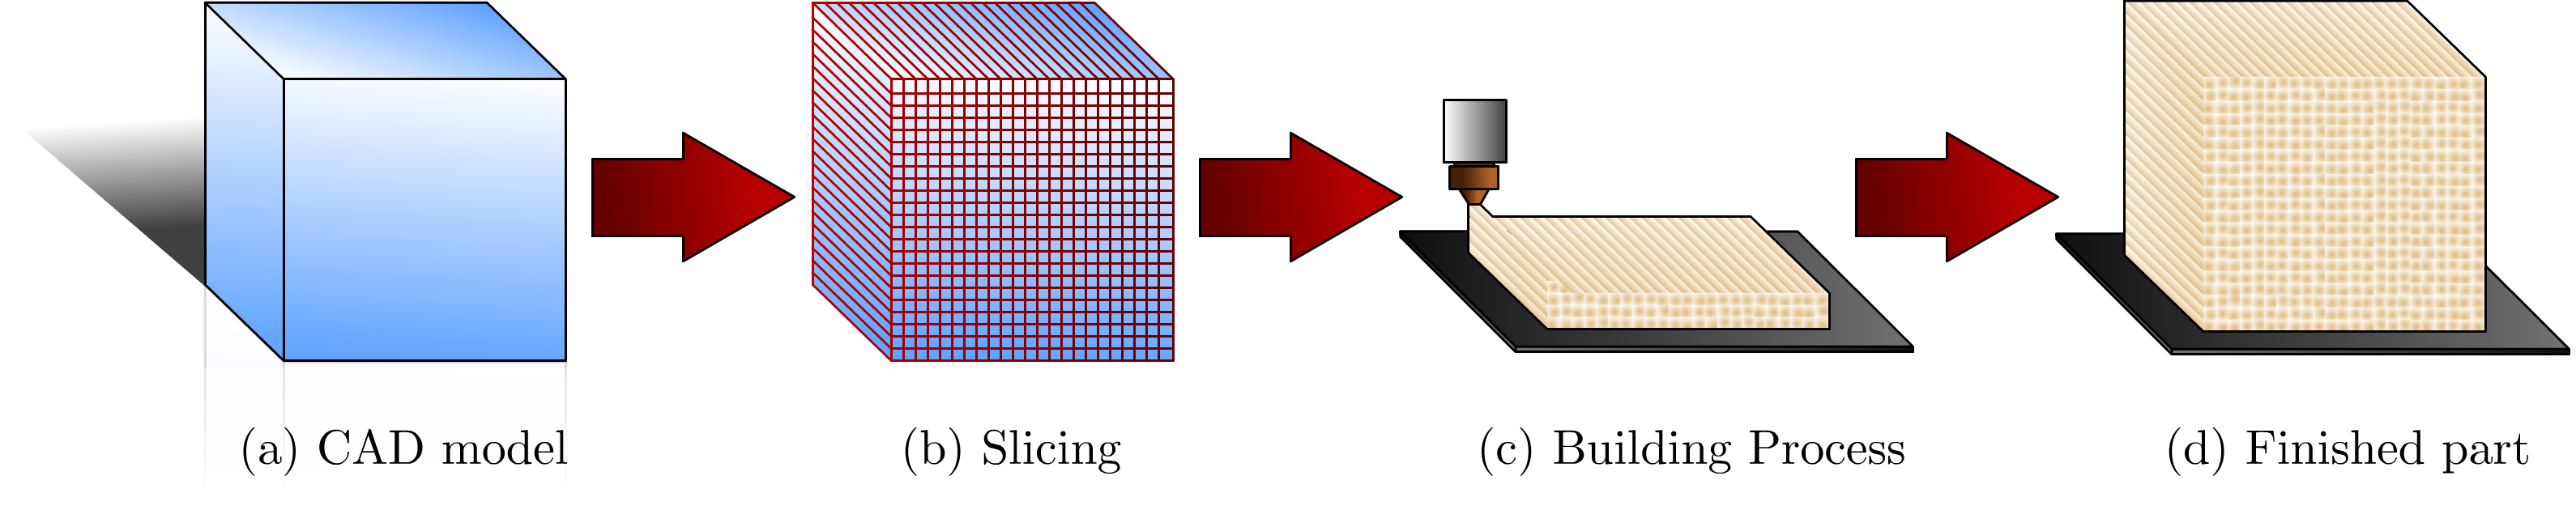
\includegraphics[width=\linewidth]{AM_flowchart_1}
	\caption{Process flow of AM} \label{fig:AM_flow}
\end{figure}
\pagebreak %Used to move the entire paragraph to a new page.
 
While all AM technologies operate on the same basic process flow described above, the specifics of each AM technique vary substantially, ranging from processes that use paper and binder, all the way through metal-based, laser tracing technologies. Since this is a rapidly evolving field, no general consensus exists for classifying the multiple AM processes available as of the time of this writing. However, the classification system proposed under the ASTM/ISO 52900 standard \cite{ASTM52900}, has been somewhat accepted by the field and divides AM technologies as follows:
\begin{enumerate}
	\item \textbf{Binder Jetting}: AM techniques where a binding agent is used to selectively promote cohesion in powder materials -generally gypsum, sand or metallic powders~\cite{ASTM52900,3DHubs2018}.
	\item \textbf{Directed Energy Deposition}: AM processes where a focused thermal energy source (i.e. laser, electron beam, plasma arc) is used to fuse materials as they are being deposited in the build volume. Materials are almost exclusively metals~\cite{ASTM52900,3DHubs2018}.
	\item \textbf{Material Extrusion}: In this type of AM technology, material is dispensed through a nozzle or orifice. Fused Filament Fabrication belongs to this classification. Materials are almost exclusively thermoplastics \cite{ASTM52900,3DHubs2018}.
	\item \textbf{Material Jetting}: AM techniques where build material is deposited selectively in droplets. Materials are usually wax or thermoplastics, but there are examples of metal-based, material jetting techniques \cite{ASTM52900,3DHubs2018}.
	\item \textbf{Powder Bed Fusion}: AM processes where portions of a powder bed are selectively fused through application of thermal energy. \emph{Selective Laser Sintering} (SLS) belongs to this category. Materials are usually thermoplastic polymers or metals \cite{ASTM52900,3DHubs2018}. 
	\item \textbf{Sheet Lamination}: In this type of AM technology, the final part is formed by bonding sheets of material -usually paper or composites \cite{ASTM52900,3DHubs2018}. 
	\item \textbf{Vat Photopolymerization}: In this AM process, a liquid photopolymer is selectively cured by a light source. \emph{Stereolithography} (SLA), arguably the first AM technology, belongs to this category. Due to the nature of this technique, the only materials used are photopolymers \cite{ASTM52900,3DHubs2018}.
\end{enumerate} 

\subsection{Advantages and Disadvantages of AM}\label{subsec:AMAdDis} 
Since AM processes allow a relatively direct conversion of a CAD model into a constructed object, they were originally exclusively used for prototype development. For this reason, they were initially classified as \textquotedblleft \emph{Rapid Prototyping}\textquotedblright~(RP) technologies. This terminology is still used today, however, it is being superseded by \emph{Additive Manufacturing} since its potential to become a proper fabrication technique exists \cite{Gibson2015}. While being capable of quickly jumping from part design to manufacturing is a great advantage, AM has its own set of drawbacks. Table \ref{tab:AM_AdDis} summarizes the most noteworthy set of advantages and disadvantages typical of most AM technologies.

\begin{table}[h]
	\centering
	\caption{Advantages and Disadvantages of Additive Manufacturing}
	\label{tab:AM_AdDis}
	\begin{tabu} to 0.95\textwidth {  X[c]  X[c] }
		\hline
		\textbf{Advantages} & \textbf{Disadvantages} \\ 
		\hline
		Faster product development cycles \cite{Gibson2015} & Part quality highly dependent on process parameters \cite{Gibson2015}\\
		%---------
		No additional tools needed for part fabrication\cite{Gibson2015}&  Stratified build generally results in anisotropic parts \cite{Gibson2015, Capote2017}\\
		%---------
		Cost effective for small batches of parts \cite{Baumers2016,Conner2014,Berman2012}&  Costly for production of more than hundreds of parts \cite{Baumers2016,Conner2014,Berman2012}\\
		\hline
	\end{tabu}
\end{table}   

Out of all advantages and disadvantages described, the high anisotropy of AM parts is responsible for the slow embrace of AM in highly demanding engineering fields -such as the aerospace and automotive industries. The highly anisotropic mechanical behavior makes it extremely difficult to predict part failure, therefore, it cannot be implemented in engineering applications where catastrophic failure is to be avoided at all costs. Even so, success stories of implementation of AM in industrial environments are abundant. Relatively recent examples include the use of FFF machines to manufacture tools, jigs, and fixtures in a Volkswagen assembly plant in Europe \cite{deVries2017}; production of a complex fuel nozzle injector for the LEAP jet engine, using powder based, metal AM by GE \cite{GEAdditive2016}; and development and production of highly optimized, 3D printed midsoles for high performance running sneakers by companies as large as New Balance and Adidas \cite{NewBalance2016,Matisons2015,Saunders2018}. Note that in the cases presented, the main reason behind the usage of AM was either reduction of expenses associated with producing small batches of parts, or the capability of reproducing a unique and complex geometry. This is a trend that is observed in most of the literature describing implementation of AM into industrial scenarios.

While the advantages and disadvantages described here cover the field of AM as a whole, each technique comes with its own set of pros and cons that may make it the preferred method to reproduce a particular product or geometry. This work, however, focuses solely on FFF. The specifics of this process are described in detail in Section~\ref{sec:FFF}.

\section{Fused Filament Fabrication}\label{sec:FFF} 
\emph{Fused Filament Fabrication}~(FFF) is an AM technology where the final geometry of the part is obtained through controlled extrusion of a liquid, self-hardening material -usually a thermoplastic polymer in molten state \cite{Gibson2015}. Originally developed by Stratasys in the 1980s under the still trademarked ~\emph{Fused Deposition Modeling}~(FDM\texttrademark) moniker, it has recently become one of the most widely used AM techniques due to the advent of low-cost, desktop FFF machines in the early 2010s caused by the expiration of key patents from Stratasys \cite{Gibson2015,Capote2017}. 

\subsection{The FFF process}\label{ssec:FFFmach}
At its core, the typical FFF machine consists of a heated build surface commonly referred to as a \emph{build plate}, a specialized tool known as a \emph{printhead}, and the fabrication material -supplied in the form of spools of thermoplastic polymer filament. The printhead is itself composed of a heating element, a nozzle, and some form of driving mechanism that pushes the filament downward. As the thermoplastic material is moved through the heated chamber, polymer melt is formed and extruded through the opening at the tip of the nozzle, producing a \emph{bead}. The molten polymer can then be deposited upon the build plate, where controlled movements of the printhead and the fabrication surface gradually construct the final geometry of the part in a layer-by-layer build approach~\cite{Gibson2015}. The typical setup of an FFF machine can be seen in Figure \ref{fig:machconfig}. In this example, the printhead moves in the \emph{x-y} plane, while the build plate moves in the \emph{z} direction. 
 
\begin{figure}[h]
	\center
	\subfloat[FFF printhead cross section\label{fig:FFFnoz}]{%
		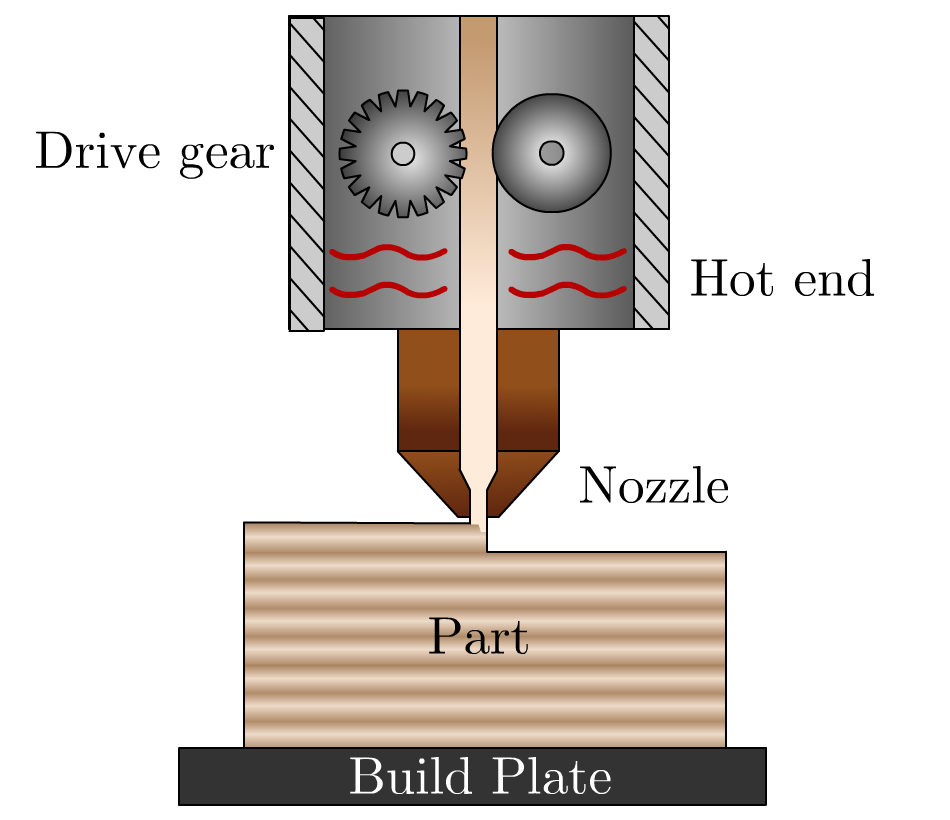
\includegraphics[height=6cm, keepaspectratio]{nozzle}
		}
	\hfill
	\subfloat[Typical FFF machine\label{fig:FFFmach}]{%
		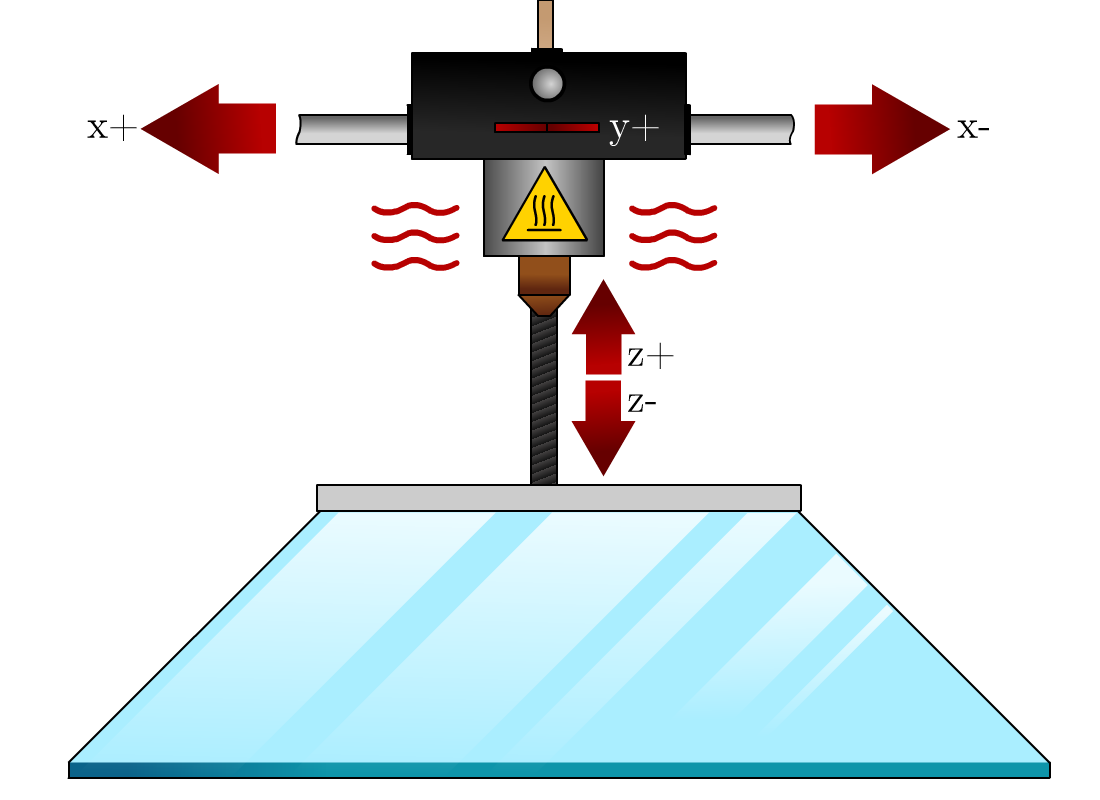
\includegraphics[height=6cm, keepaspectratio]{printer_layout}
		}
	\caption{The basic FFF machine configuration} \label{fig:machconfig}
\end{figure}
Like all AM technologies, the FFF process starts in a computer with a CAD model converted to the \emph{.stl} file format. The geometry is then translated to machine instructions through a \emph{slicing engine}, where the user inputs a plethora of process parameters that include nozzle and build plate temperatures, print speed, layer thickness, and build orientation. Finally the \emph{toolpath} is executed by the FFF printer, building the object in a layer-by-layer basis \textendash~sometimes referred to as \emph{2.5D} printing~\cite{Gibson2015, VanHulle2017}. Figure \ref{fig:FFFflow} shows an abridged version of the process. The \emph{z} axis indicates the intended build direction. Note how some of the finer details in the original CAD file are lost in the printed part \textendash~due in part to the layer height and build orientation selected.

\pagebreak
\begin{figure}[h]
	\center
	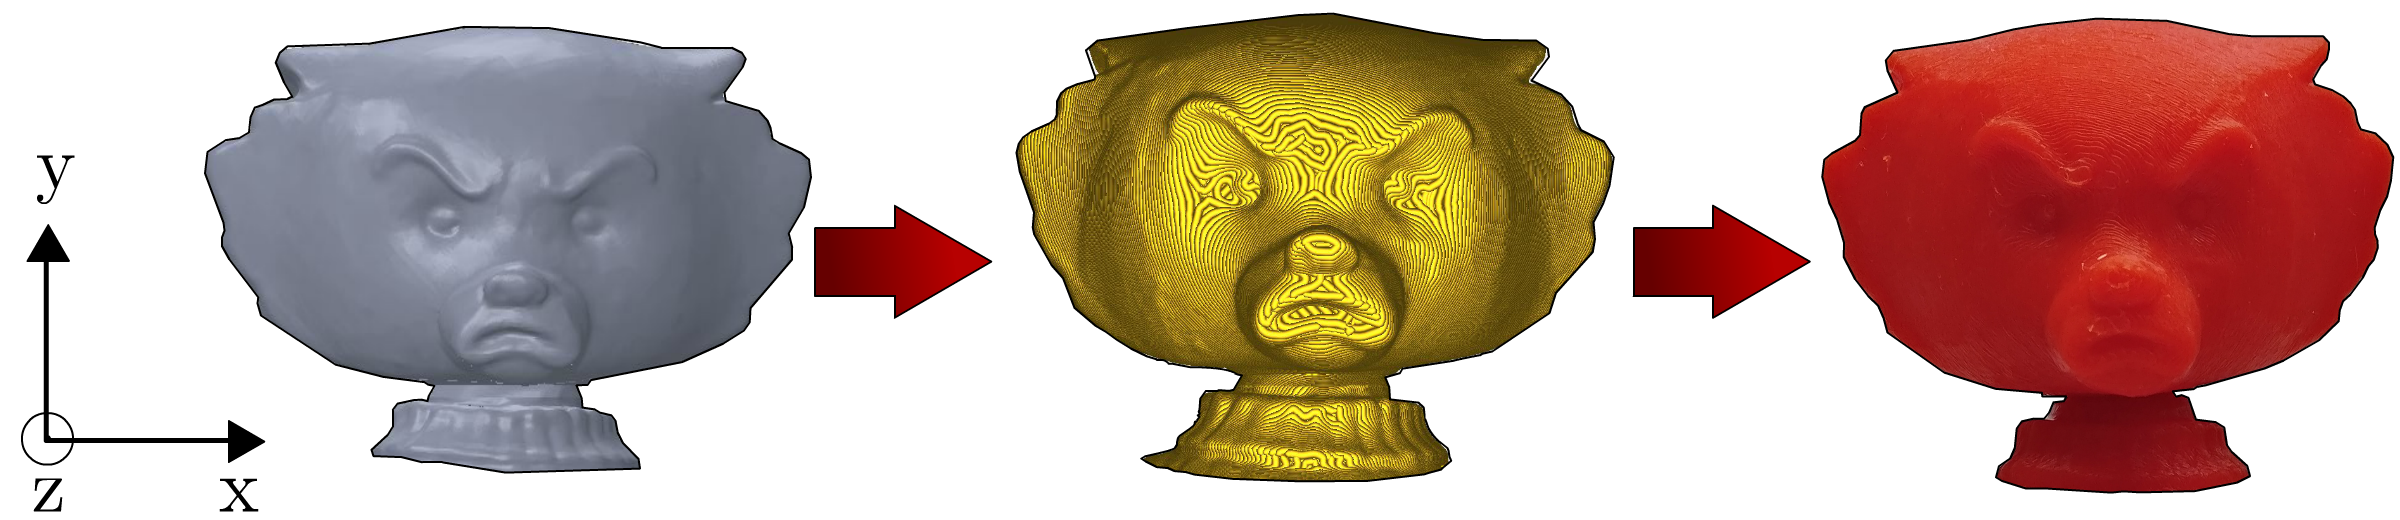
\includegraphics[width=0.95\textwidth]{FFFflow}
	\caption{Model, toolpath and final part in the FFF process} \label{fig:FFFflow}
\end{figure}

The process is capable of producing complex geometries that would be otherwise hard to reproduce through other polymer processing techniques, such as injection molding. However, it is bound by the disadvantages described in Section \ref{subsec:AMAdDis}, as well its own unique set of drawbacks. Namely:

\begin{itemize}
	\item The circular orifice in the nozzle makes FFF incapable of reproducing sharp corners, limits the size of the smallest reproducible feature, and causes the final part to be filled with voids \textendash originating in the junction of round beads. These problems can be seen in Figure \ref{fig:FFFpartprob}: On the left, a comparison of a 90$^\circ$ corner planned in the toolpath and the final geometry of the printed bead is shown. Note the rounded nature of the turn. On the right, a cross section of an FFF part obtained through \emph{Micro Computer Tomography} ($\mu$CT) shows the voids that form during the printing process.
	\begin{figure}[h]
		\center
		\subfloat[FFF toolpath vs. printed bead\label{fig:FFFbead}]{%
			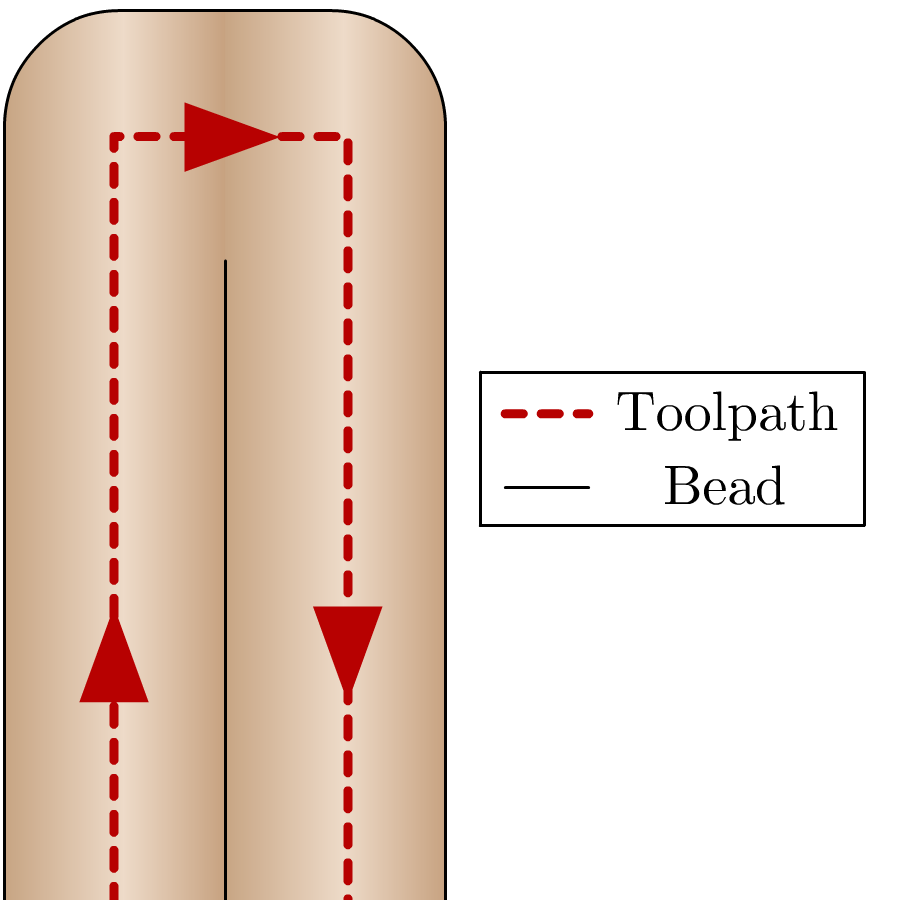
\includegraphics[height=6cm, keepaspectratio]{Toolpath}
		}
		\hfill
		\subfloat[Cross section of an FFF part\label{fig:FFFuCT}]{%
			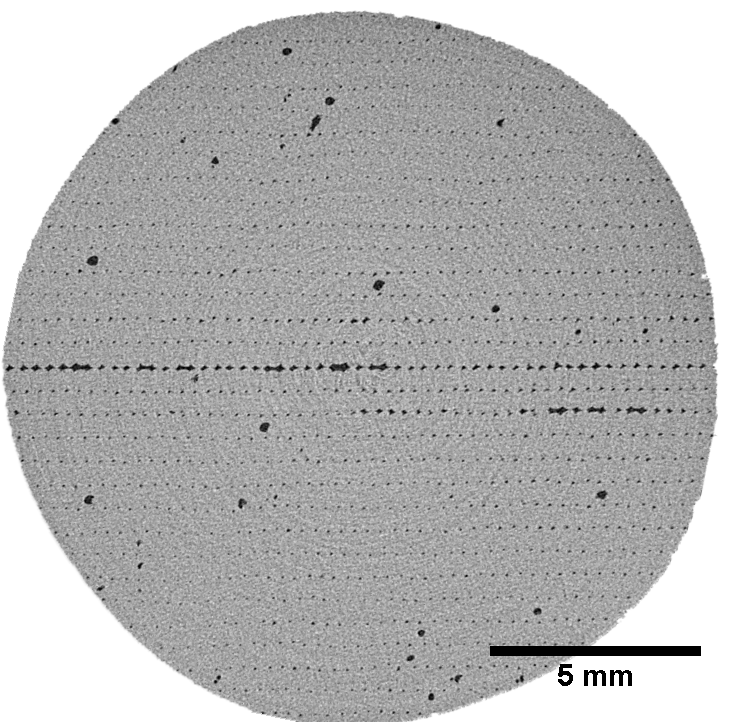
\includegraphics[height=6cm, keepaspectratio]{uCT_FFF}
		}
		\caption{Typical FFF part mesostructure and its origin} \label{fig:FFFpartprob}
	\end{figure}
	\item The junction of adjacent beads behaves akin to a polymeric weld, and has inferior mechanical properties than the bulk material \cite{Capote2017}. This, coupled with the aforementioned voids which can act as stress concentrators, causes FFF parts to behave in extremely anisotropic manner with diminished mechanical performance when compared to analogous parts obtained through traditional polymer processing technologies \textendash~such as injection molding \cite{Capote2017}.
\end{itemize}

This last disadvantage is responsible for the slow embrace of FFF as a proper manufacturing technique: the high anisotropy of FFF parts imply that predicting part failure becomes extremely difficult and thus, proper part design that guarantees safe operation of the object under important loads is hard to achieve.  For this reason, efforts to characterize the mechanical behavior of FFF parts have existed since as early as the 1990s. Recent examples are presented in Section \ref{ssec:mechPropFFF}.

\subsection{Mechanical Properties of FFF parts}\label{ssec:mechPropFFF}

Efforts have been made to characterize the mechanical anisotropy of FFF parts. However, due to the lack of testing standards and problems during toolpath planning, most studies focus solely in the tensile mechanical performance of FFF coupons.

Studies performed by Koch \emph{et al.} \cite{Koch2017} and Rankouhi \emph{et al.} \cite{Rankouhi2016} indicate that the final tensile properties of FFF coupons are particularly sensitive to bead orientation and proper mass output through the nozzle. Other process parameters, such as the layer thickness, have varying degrees of impact upon the final tensile strength of the part. In both studies, tensile coupons were printed with bead orientations of 0$^\circ$, 45$^\circ$ and 90$^\circ$ in the \emph{x-y} plane. Results showed that in all the experimental conditions selected, a 0$^\circ$ orientation always behaved closer to the bulk material, whereas a 90$^\circ$ sample always had significantly lower tensile strengths. The 45$^\circ$ samples sat between both extremes. It is important to note that in both studies, toolpath manipulation was necessary to avoid premature failure of the coupons due to stress concentrators originating in void formation due to the elliptical nature of the beads. Figure \ref{fig:FFFmechProp} shows some of the results by Koch \emph{et al}. The geometry corresponds to an ASTM Type I Tensile coupon. Injection molded results are denoted \emph{IM} for comparison. Note that the 90$^\circ$ orientation had a tensile strength that was 25\% inferior to the IM counterpart, and 20\% worse than the 0$^\circ$ oriented FFF coupon. This is a prevalent trend in the consulted bibliography.

Literature for other types of mechanical testing of FFF parts is relatively scarce when compared to tension experiments. Research indicates that the compressive strength of FFF parts tends to be higher than the tensile strength, as well as being less sensitive to process parameters \textemdash the bead orientation in particular seems to have a significantly diminished impact upon the compressive strength when compared to its effect upon tensile tests \cite{Ahn2002,Lee2007}. Shear strength results are virtually non-existent.

\pagebreak
\begin{figure}[h]
	\center
	\subfloat[Tensile strength of tensile coupons\label{fig:KochCoup}]{%
		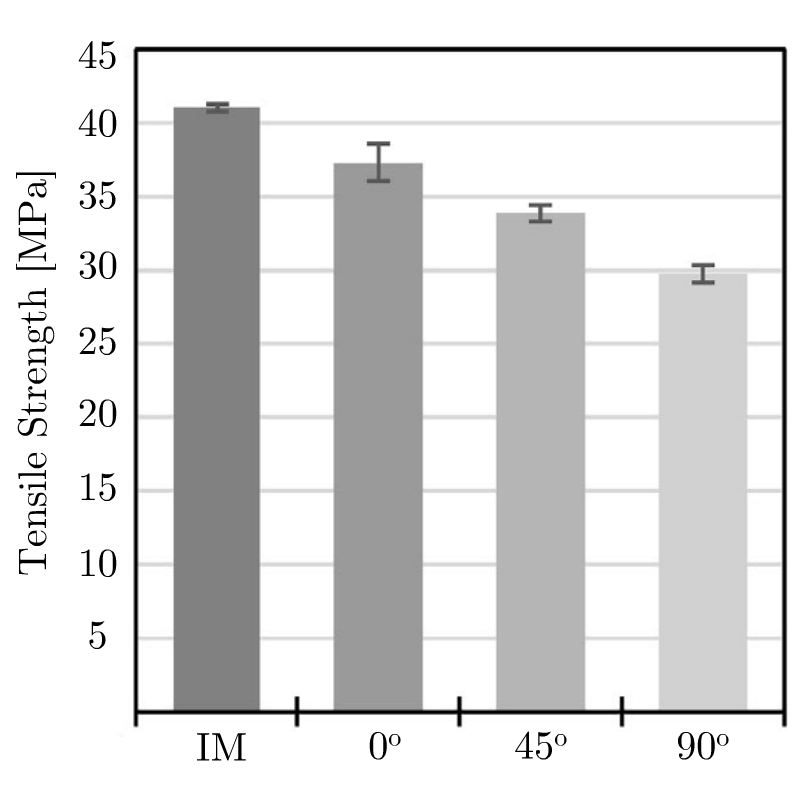
\includegraphics[height=6cm, keepaspectratio]{lit_mechpropFFF}
	}
	\hfill
	\subfloat[Representation of coupons used\label{fig:KochRes}]{%
		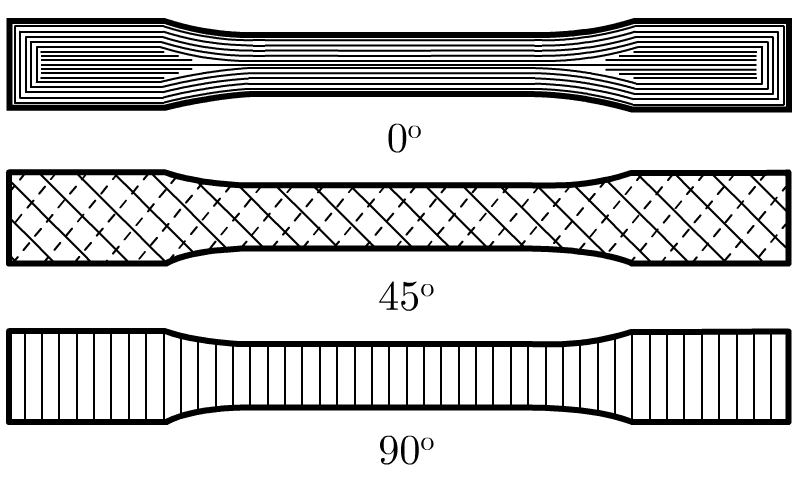
\includegraphics[height=4cm, keepaspectratio]{lit_mechpropFFF2}
	}
	\caption{Results from Koch \emph{et al.} \cite{Koch2017}} \label{fig:FFFmechProp}
\end{figure}

\section{Failure Criteria}\label{sec:FC}   
The increased use of advanced materials in industry has brought upon a necessity to properly characterize their strengths and failure modes. Composites in particular are commonly used in highly demanding engineering fields given that they excel in mechanical properties. However, due to their nature, their behavior is extremely anisotropic. For this reason, it has been of great interest to develop a proper way to model the behavior of anisotropic materials under mechanical stresses as a way to predict part failure \textendash~a practice from here on referred to as developing a \emph{failure criterion}. 

Early attempts to properly predict failure of anisotropic materials go as far back as 1948 with the Hill model \cite{Osswald2017a}. Further developments led to a plethora of Failure Criteria (FC), such as the Tsai-Hill, Malmeister, Tsai-Wu, Gol'denblat-Kopnov, Puck, and Cuntze to name a few \cite{Osswald2017a,Osswald2015}. A wide variety of criteria exists because a model will rarely capture the complete failure behavior of an anisotropic material. To illustrate this point, refer to Figure \ref{fig:FCComp}, reproduced from work by Sun \emph{et al}. \cite{Sun1996} where a composite glass fiber and epoxy laminate was loaded biaxially, in a direction that was either parallel ($\sigma_{11}$), perpendicular ($\sigma_{22}$) to the fiber, or a combination of both. Positive stresses indicate tensile load, while negative values point to compressive forces. The data, represented by the white squares, does not agree with any of the used models in the fourth quadrant of the graph. This type of behavior is common throughout the literature: Puck's model is great at predicting shear strengthening effects, but doesn't perform well when dealing with combined axial loading scenarios; the Gol'denblat-Kopnov model by contrast is great at predicting axial stress interactions, but falls short when dealing with shear strengthening effects caused by combined shear-axial loadings. These trends point to the limitations of each model: in order to either facilitate calculations, or due to the difficulty of performing combined loading tests, interaction effects are neglected either by mathematical choice, or indirectly through the inner workings of the failure criterion \cite{Osswald2017a}.  

\begin{figure}[h]
	\center
	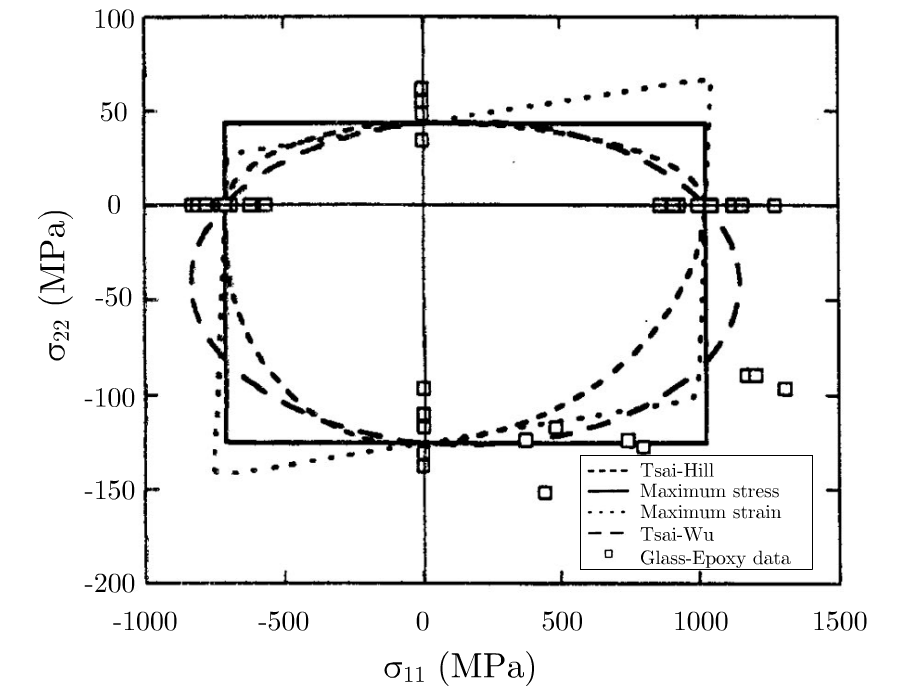
\includegraphics[height=10cm, keepaspectratio]{FC_comparison}
	\caption{Comparison of different failure criteria. \cite{Sun1996}} \label{fig:FCComp}
\end{figure}     

\subsection{The Stress-Stress Interaction Criterion}

The majority of FC fail to completely integrate interaction effects into the modeled failure behavior of anisotropic materials. Work published in 2017 by Paul and Tim Osswald \cite{Osswald2017a} proposed a model that attempts to overcome these limitiations by developing a failure function based on the approach described by Gol'denblat and Kopnov in 1965 \cite{Goldenblat1965}. The model proposed by Osswald and Osswald, originally titled \textquotedblleft A Strength Tensor Based Failure Criterion with Stress Interactions\textquotedblright, will be referred in this work as the Stress-Stress Interaction Criterion (SSIC), and has the following characteristics:

\begin{itemize}
	\item \textbf{Tensor based and purely mathematical}: as opposed to phenomenological or mechanistic models such as the Puck or Cuntze failure criteria.
	\item \textbf{Includes stress interactions that other models neglect}.
\end{itemize}

To understand the SSIC, it is necessary to describe the model upon which it is based. The Gol'denblat-Kopnov Criterion (GKC) describes a mathematical function that depends on the stress state of an anisotropic material. Should the computation of this expression exceed a threshold, part failure is to be expected. To that end, a scalar function that depends on stress tensors that completely characterize the state of the material was developed \cite{Goldenblat1965}. This function is shown in Equation \ref{eq:GKCgen}, where stresses are denoted $\sigma$, and the subindices \emph{i,j,k,l} denote a particular load direction.

\begin{equation} \label{eq:GKCgen}
f=(F_{ij}\sigma_{ij})^\alpha + (F_{ijkl}\sigma_{ij}\sigma_{kl})^\beta + (F_{ijklmn}\sigma_{ij}\sigma_{kl}\sigma_{mn})^\gamma + ...
\end{equation}

The terms $F_{ij}$, $F_{ijkl}$ and $F_{ijklmn}$ represent second, fourth and sixth order tensors respectively. These terms of the equation depend on engineering strength parameters, such as the ultimate tensile and compressive strengths of the material in a particular load direction \cite{Osswald2017a}. Due to the complexity associated with using higher order tensors, Gol'denblat and Kopnov limited their approach to using only the second and fourth order terms. Thus Equation \ref{eq:GKCgen} is reduced to:

\begin{equation} \label{eq:GKCgenTrunc}
f=(F_{ij}\sigma_{ij})^\alpha + (F_{ijkl}\sigma_{ij}\sigma_{kl})^\beta
\end{equation}

In order to attain a linear criterion scalar function, the exponents $\alpha$ and $\beta$ were assigned values of 1 and 1/2 respectively. Finally, in plane stress scenarios, the GKC becomes:

\begin{equation} \label{eq:GKCfinal}
\begin{split}
f=F_{11}\sigma_{11} + F_{22}\sigma_{22} + F_{12}\tau_{12} + (F_{1111}\sigma_{11}^{2} + F_{2222}\sigma_{22}^{2} + F_{1212}\tau_{12}^{2} \\ + 2F_{1122}\sigma_{11}\sigma_{22} + 2F_{1112}\sigma_{11}\tau_{12} + 2F_{2212}\sigma_{22}\tau_{12})^{1/2}
\end{split}
\end{equation}

Note that in Equation \ref{eq:GKCfinal} $\sigma$ and $\tau$ denote normal and shear stresses respectively. Figure \ref{fig:loaddir} depicts an anisotropic material and all the possible loading directions for reference.

\begin{figure}[h]
	\center
	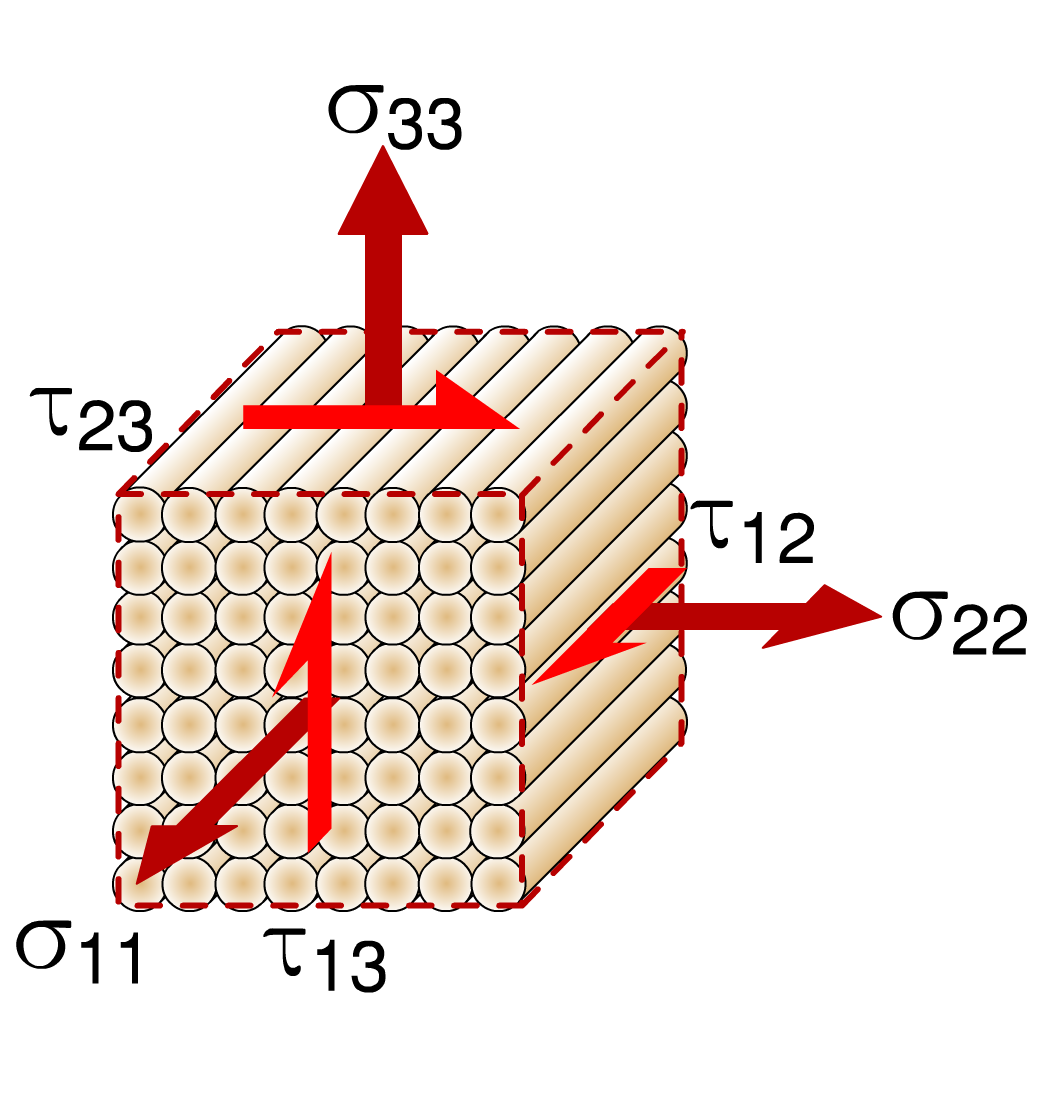
\includegraphics[height=5cm]{reference_cube}
	\caption{Different load directions in an anisotropic material} \label{fig:loaddir}
\end{figure}

Per Gol'denblat and Kopnov's design, should the computation of $f$ in Equation \ref{eq:GKCfinal} be greater or equal to 1, part failure is to be expected. However, to simplify calculations, they deliberately assumed the interaction terms $F_{1112}$ and $F_{2212}$ to be zero. This is an important consideration that will come into play when describing the SSIC.

Most of the terms in the GKC are obtained through mechanical testing of coupons under pure uniaxial loads in the 1 or 2 direction, or pure shear in the 1-2 plane \cite{Osswald2017a}. In these scenarios, $f$ will be equal to 1 at failure, and the stress state will be known to the user, allowing some of the unknown tensorial parameters to be easily calculated. Using $F_{11}$ and $F_{1111}$ as examples, the process would be as follows:


\begin{enumerate}
	\item The tensile and compressive strength in the 1-1 direction would be obtained through mechanical testing. These values are named $X_t$ and $X_c$ respectively.
	\item Under these failure conditions, Equation \ref{eq:GKCfinal} is reduced to the following system of equations:
	\[
	\systeme*{1=F_{11}X_t + (F_{1111}X_t^{2})^{1/2}, 1= -F_{11}X_c + (F_{1111}X_c^{2})^{1/2}}
	\]
	
	\item $F_{11}$ and $F_{1111}$ can be obtained, yielding $F_{11}=\frac{1}{2}(\frac{1}{X_t}-\frac{1}{X_c})$ and $F_{1111}=\frac{1}{4}(\frac{1}{X_t}+\frac{1}{X_c})^2$.
\end{enumerate}

The only exception to this procedure would be the $F_{1122}$ component, which requires measuring the positive and negative shear strengths of a coupon with reinforcement oriented in 45$^\circ$. These parameters are named $S_{45p}$ and $S_{45n}$ respectively. Table \ref{tab:GKparam} summarizes the nomenclature used for the strength parameters required to completely populate the failure function of the GKC. Table \ref{tab:GKtens} summarizes all the tensorial component calculations.

\begin{table} [h]
	\centering
	\caption{Nomenclature of the GKC parameters}
	\begin{tabular}{ c c }
		\toprule
		\textbf{Parameter} & \textbf{Description} \\ 
		\midrule
		$X_t$ & Tensile strength in the 1-1 direction\\
		$X_c$ & Compressive strength in the 1-1 direction\\
		$Y_t$ & Tensile strength in the 2-2 direction\\
		$Y_c$ & Compressive strength in the 2-2 direction\\
		$S_{45p}$ & Positive shear strength for 45$^\circ$ specimen\\
		$S_{45n}$ & Negative shear strength for 45$^\circ$ specimen\\
		$S$ & Shear strength in the 1-2 plane\\
		\bottomrule
	\end{tabular}
	\label{tab:GKparam}
\end{table}

\begin{table} [h]
	\centering
	\caption{Tensorial components of the GKC}
	\begin{tabular}{ c c } 
		\toprule
		\textbf{Component} & \textbf{Formula} \\
		\midrule
		$F_{11}$ & $\frac{1}{2}(\frac{1}{X_t}-\frac{1}{X_c})$\\ [1ex]
		$F_{1111}$ & $\frac{1}{4}(\frac{1}{X_t}+\frac{1}{X_c})^2$\\ [1ex]
		$F_{22}$ & $\frac{1}{2}(\frac{1}{Y_t}-\frac{1}{Y_c})$\\ [1ex]
		$F_{2222}$ & $\frac{1}{4}(\frac{1}{Y_t}+\frac{1}{Y_c})^2$\\ [1ex]
		$F_{12}$ & 0\\ [1ex]
		$F_{1212}$ & $\frac{1}{S^2}$\\ [1ex]
		$F_{1122}$ & $\frac{1}{8}[(\frac{1}{X_t}+\frac{1}{X_c})^2+(\frac{1}{Y_t}+\frac{1}{Y_c})^2-(\frac{1}{S_{45p}}+\frac{1}{S_{45n}})^2]$\\ [1ex]
		\bottomrule
	\end{tabular}
	\label{tab:GKtens}
\end{table}

One of the assumptions made in the GKC is that the components $F_{1112}$ and $F_{2212}$ in Equation \ref{eq:GKCfinal} are null. While this simplifies the model, it essentially neglects any interactions between axial loads and shear stresses, namely, the $\sigma_{11}$~-~$\tau_{12}$ and $\sigma_{22}$~-~$\tau_{12}$ interactions. Practically, this causes the failure surface developed through the GKC to under-predict shear strengthening effects exhibited by anisotropic materials loaded in combined axial and shear conditions. The Stress-Stress Interaction Criterion (SSIC) attempts to overcome these limitations by building upon the GKC. For the SSIC, the interaction effects are captured through the use of the slopes of the failure surface at any of the points where the engineering strength is known within a particular stress plane \cite{Osswald2017a}. In this failure scenario, the stress state of the coupon is known and easy to implement into Equation \ref{eq:GKCfinal}, where $f=1$. The resulting expression can then be derived with respect to one of the stresses, allowing for the interaction components to be calculated. This is better illustrated through an example. Assuming the component of interest is $F_{2212}$, the procedure to calculate it through the SSIC would be as follows:

\begin{enumerate}
	\item Obtain all the tensorial components possible through the GKC.
	\item Using the $\sigma_{22}$\textendash$\tau_{12}$ stress plane, take the derivative of Equation \ref{eq:GKCfinal} as a function of $\sigma_{22}$ in the scenario of failure under pure shear ($f=1$). This yields the expression:
	\begin{equation} \label{eq:OOCex1}
	0= F_{22}+[F_{1212}S(\frac{d\tau_{12}}{d\sigma_{22}})+F_{2212}S]
	\end{equation}
	where $\frac{d\tau_{12}}{d\sigma_{22}}$  is the slope of the graph at failure under shear. This term is named $\mu^{2212}$ in the SSIC and can be obtained by performing combined loading tests. 
	
	\item Rearranging Equation \ref{eq:OOCex1} to solve for the unknown $F_{2212}$ gives the following expression:
	\begin{equation} \label{eq:OOCex2}
	F_{2212}=-\frac{F_{22}}{S}-F_{1212}\mu^{2212}
	\end{equation}
\end{enumerate}


A similar procedure can be followed for any $\sigma_{ii}$-$\tau_{ij}$ interaction, or even any $\sigma_{ii}$-$\sigma_{jj}$ components. For this last scenario, the user has four potential choices of slopes to determine the tensorial component of interest. In the SSIC, any slope obtained from a $\sigma_{ii}$-$\sigma_{jj}$ stress plane is named $\lambda^{iijj}$, as opposed to $\mu^{iiij}$ for slopes in a $\sigma_{ii}$-$\tau_{ij}$ reference. A schematic of all possible interaction slopes is shown in Figure \ref{fig:SSICdemo}, while Table \ref{tab:OOCcomp} summarizes all the possible interaction factors available through the SSIC, where $\tau_{ij}^u$ denotes ultimate shear strength in a particular shear plane. 

\pagebreak
\begin{figure}[h]
	\center
	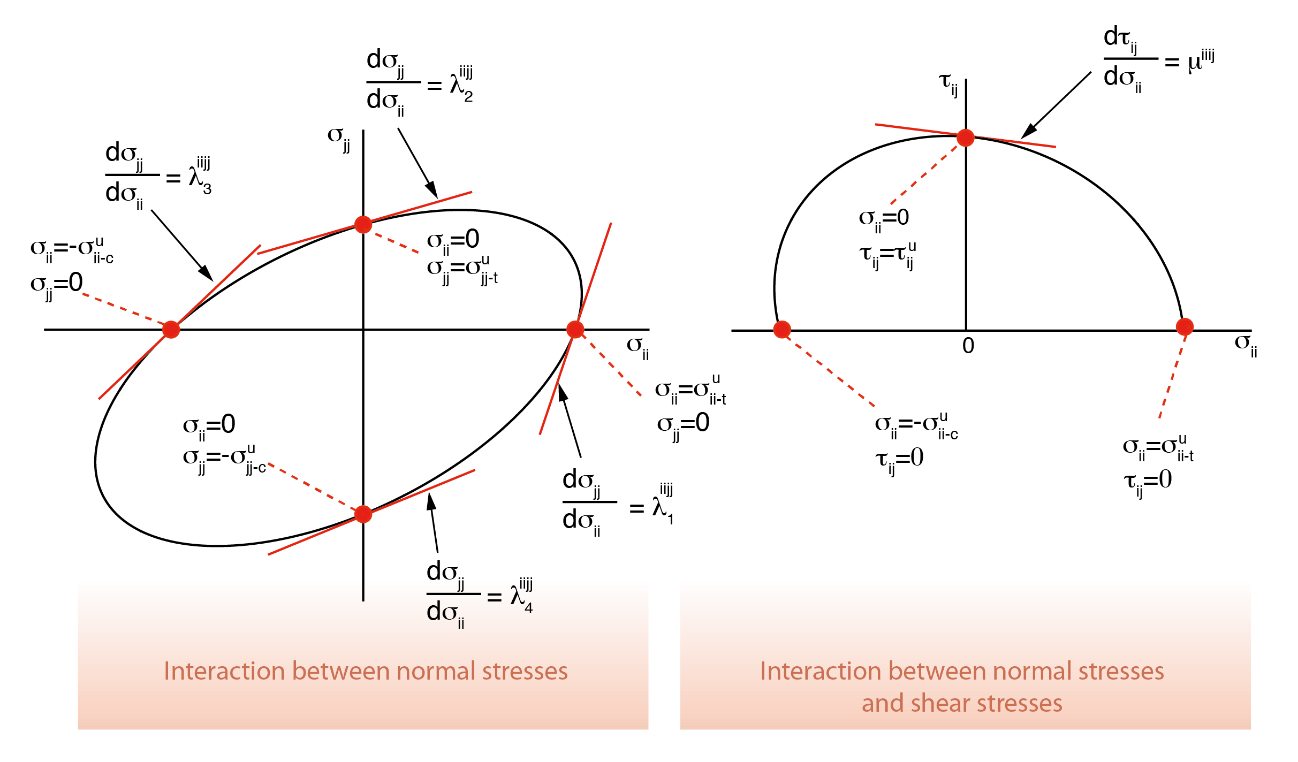
\includegraphics[height=9cm]{ssic_slopes}
	\caption{Interaction slopes available through the SSIC} \label{fig:SSICdemo}
\end{figure}
\begin{table}[!htbp] %Fixates table so that it doesn't randomly jump around between pages
	\renewcommand{\arraystretch}{1.5}
	\centering
	\caption{Interaction components attainable through the SSIC~\cite{Osswald2017a}}
	\begin{tabular}{ c c } 
		\toprule
		\textbf{Component} & \textbf{Formula} \\
		\midrule
		$F_{iiij}$ & $-\frac{F_{ii}}{\tau_{ij}^u}-F_{ijij}\mu^{iiij}$\\
		$F_{iijj}$ through $\lambda^{iijj}_1$ & $-\frac{(F_{ii}+F_{jj}\lambda^{iijj}_1)F_{iiii}^{1/2}+F_{iiii}}{\lambda^{iijj}_1}$\\
		$F_{iijj}$ through $\lambda^{iijj}_2$ & $-(F_{ii}+F_{jj}\lambda^{iijj}_2)F_{jjjj}^{1/2}-F_{jjjj}\lambda^{iijj}_2$\\
		$F_{iijj}$ through $\lambda^{iijj}_3$ & $\frac{(F_{ii}+F_{jj}\lambda^{iijj}_3)F_{iiii}^{1/2}-F_{iiii}}{\lambda^{iijj}_3}$\\
		$F_{iijj}$ through $\lambda^{iijj}_4$ & $(F_{ii}+F_{jj}\lambda^{iijj}_4)F_{jjjj}^{1/2}-F_{jjjj}\lambda^{iijj}_4$\\
		\bottomrule
	\end{tabular}
	\label{tab:OOCcomp}
\end{table}


The SSIC offers a way of capturing in a more accurate manner the different failure modes of parts produced through AM technologies. As an example, the model has been successfully implemented by Obst \emph{et al.} in 2018 for SLS manufactured parts produced with PA12 \cite{Obst2018, Obst2017}. Their results show how the model was able to capture the $\tau_{12}$-$\sigma_{22}$ and $\sigma_{11}$-$\sigma_{22}$ interactions. The failure surface obtained, shown in Figure \ref{fig:OOCSLS}, was able to capture the interactions between certain axial and transverse stresses. However, due to the limitations of the SLS process, it was not possible to measure the interaction slope between the $\tau_{12}$ and $\sigma_{11}$ directions.

\begin{figure}[h]
	\center
	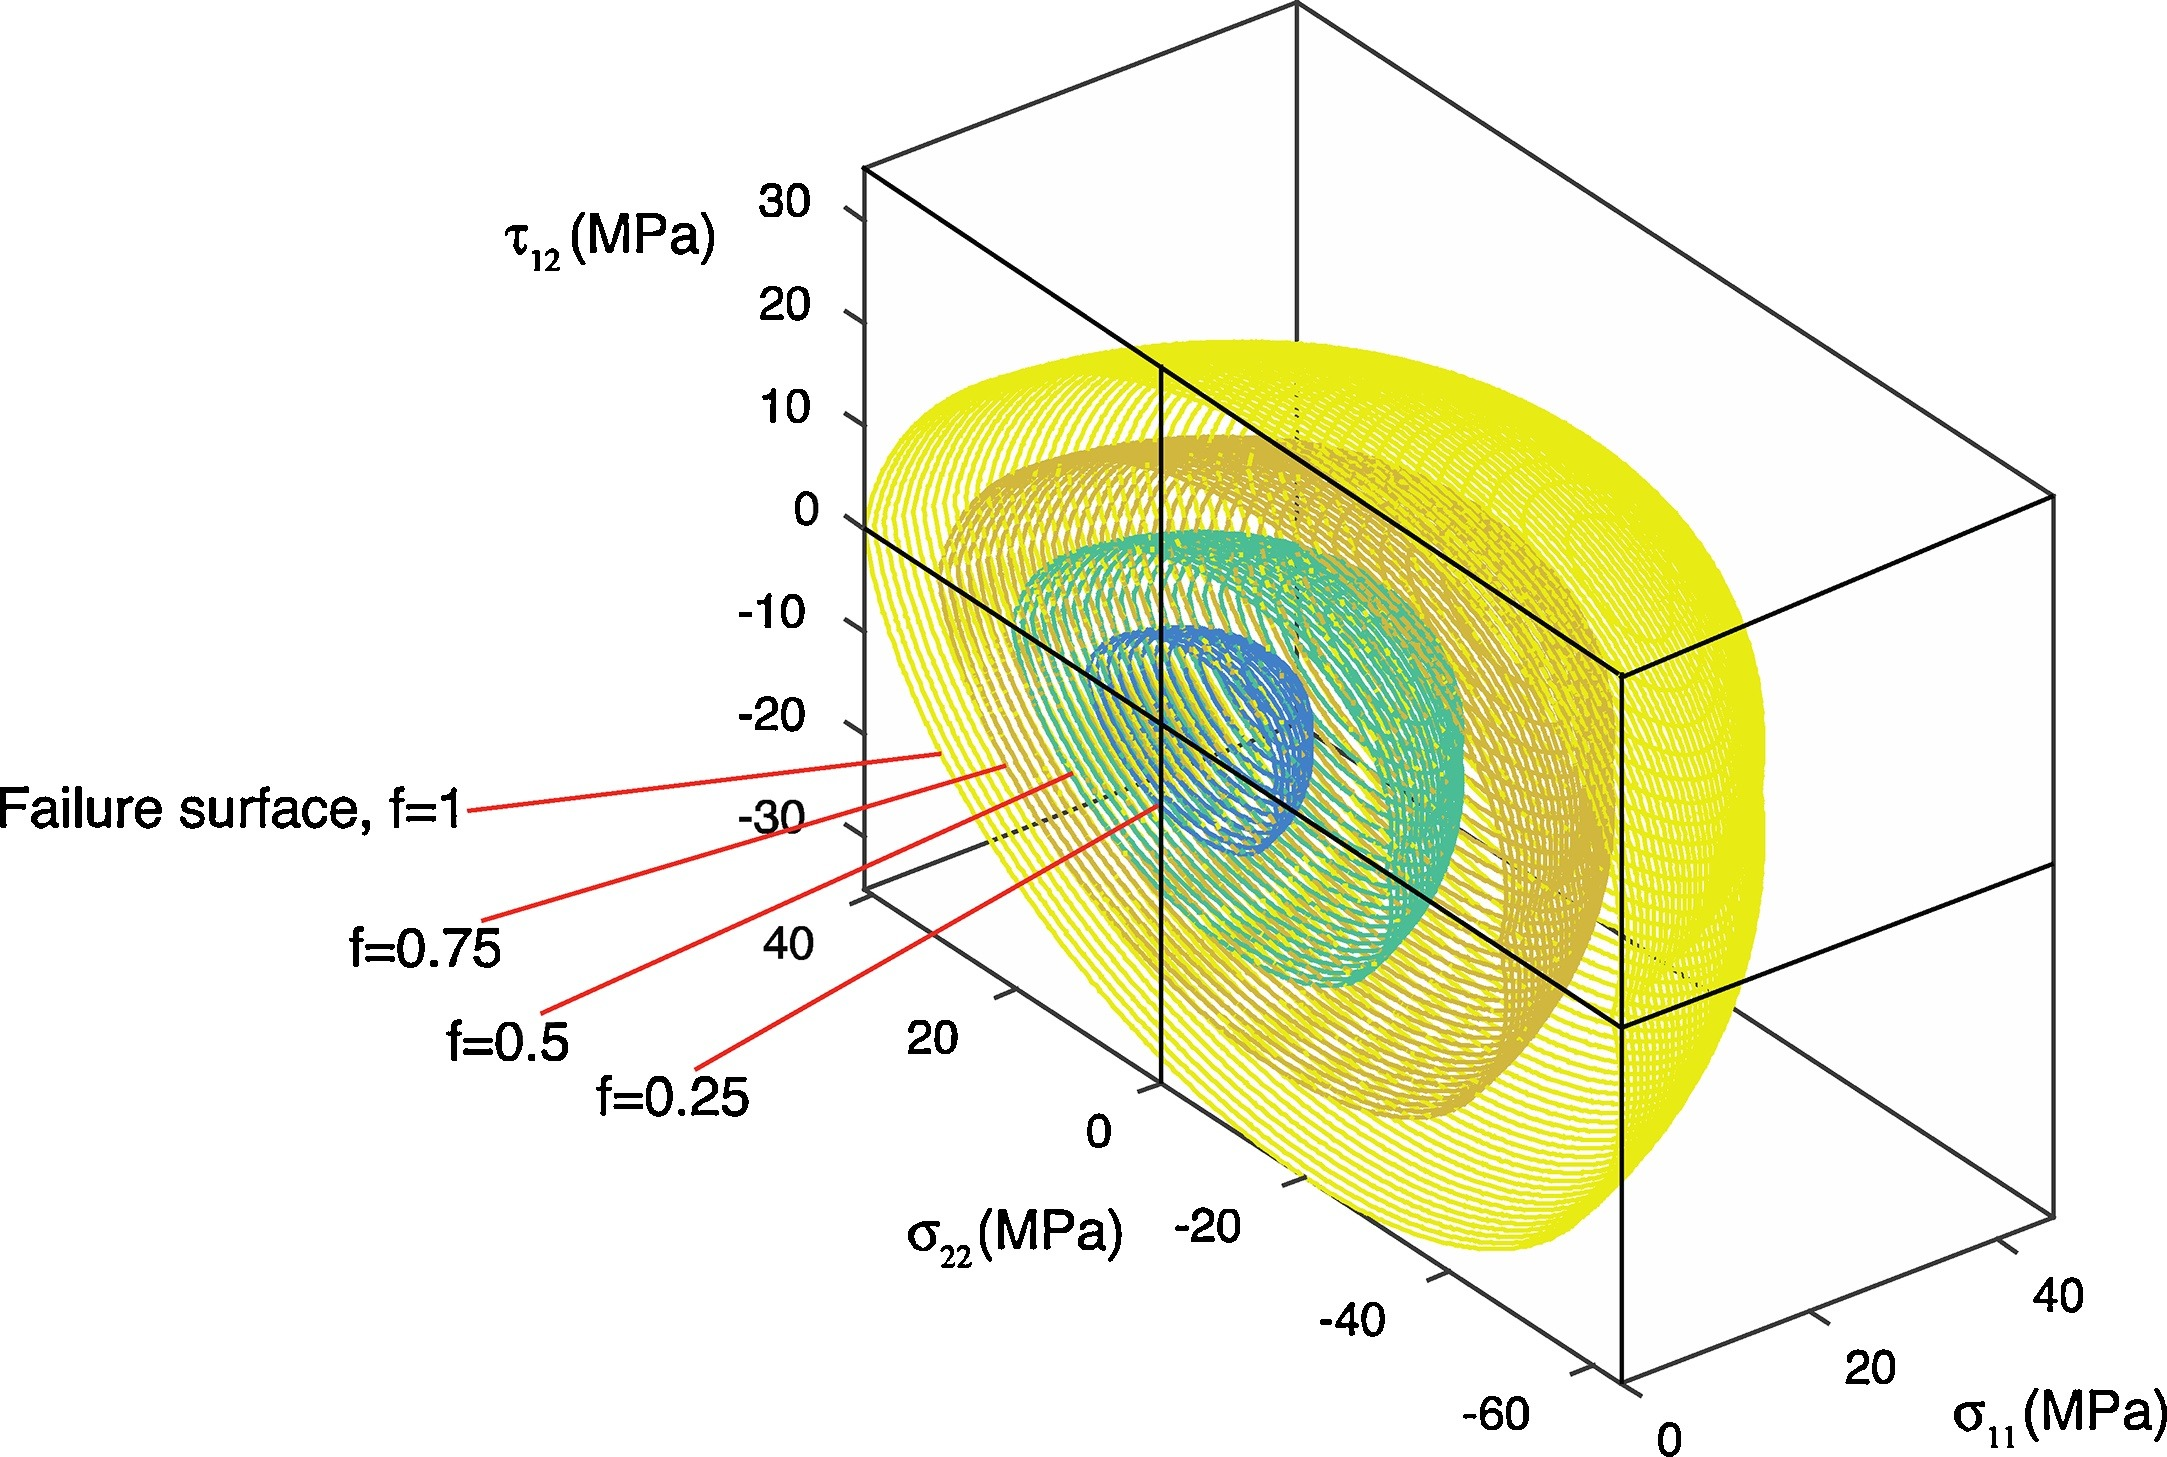
\includegraphics[height=6cm]{Obst_SLS}
	\caption{Failure surface for SLS developed through the SSIC \cite{Obst2018}} \label{fig:OOCSLS}
\end{figure}

Recent work by Osswald \emph{et al.} \cite{Osswald2020a} generated a failure envelope for Multi-Jet Fusion (MJF) parts produced using PA12, and compared it to the surface obtained by Obst \emph{et al.} \cite{Obst2018}. Results indicate that, while both techniques are based on Powder Based Fusion (PBF) and use the same material, the envelopes for each AM technology were distinct, serving as proof that these technologies are not as comparable under complex loading conditions as previously assumed. The transverse-axial interaction for the MJF case was significantly less pronounced than for SLS, further reinforcing that each AM technique needs to be studied in a case-by-case basis in terms of mechanical failure characterization. 

\begin{figure}[!htbp]
	\center
	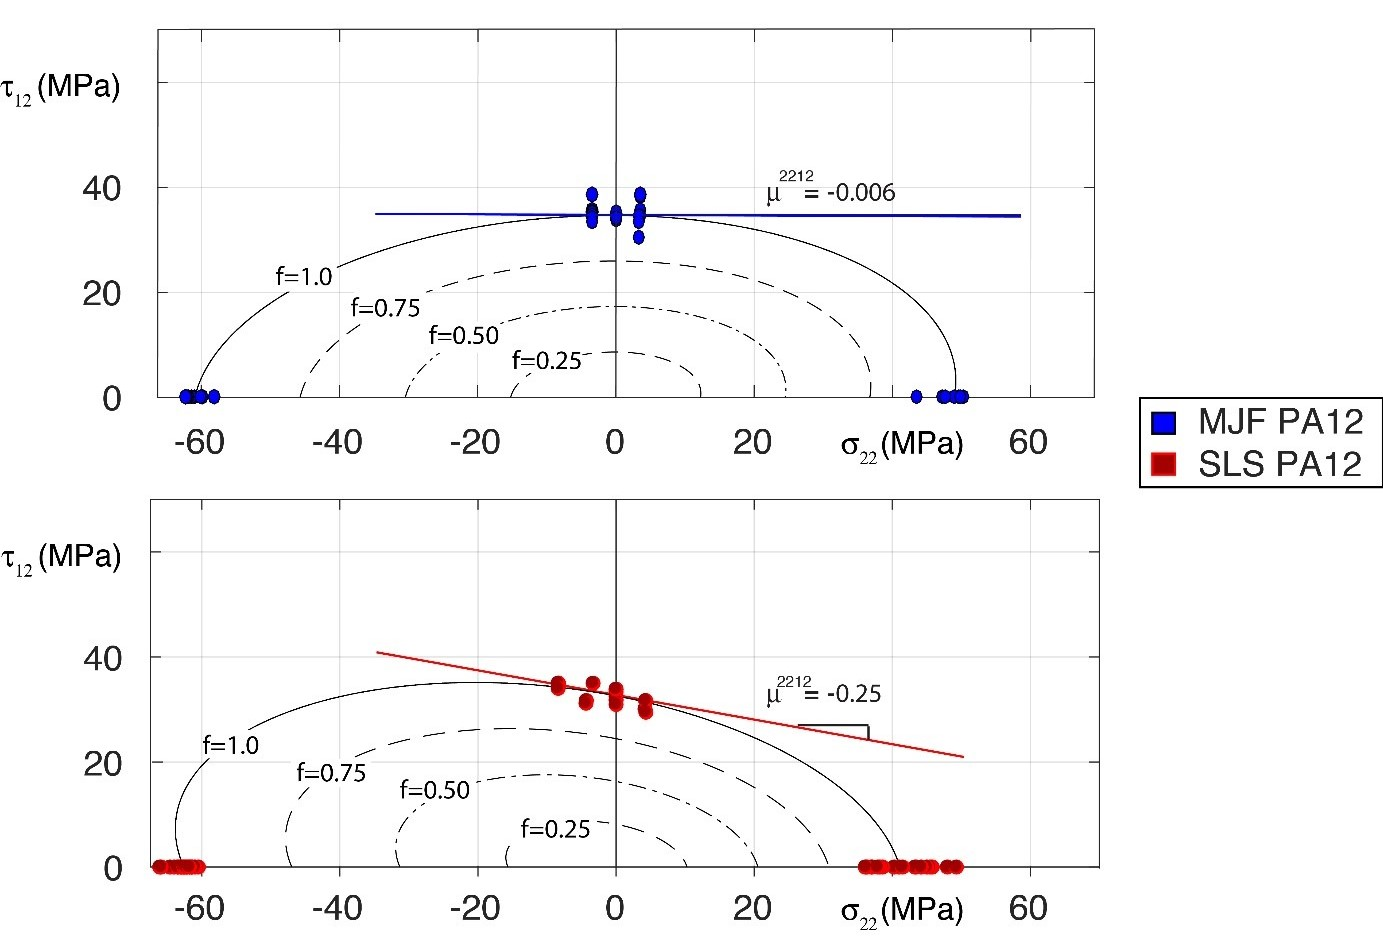
\includegraphics[height=10cm]{pbfcomp}
	\caption{Comparison of the $\sigma_{22} - \tau_{12}$ interaction for SLS and MJF PA12 parts \cite{Osswald2020a}} \label{fig:pbfcomp}
\end{figure}

\section{Development of SSIC envelope for FFF parts}\label{sec:SSICFFF}

In 2019, Mazzei Capote \emph{et al.} \cite{MazzeiCapote2019} developed a failure envelope for FFF parts produced using a customized ABS filament produced in-house. Specimens were produced using either a commercially available desktop FFF printer (Lulzbot TAZ5, USA), or a customized 6-axis robotic printing solution whenever the bead orientation was hard to achieve using a \emph{2.5-D} machine. The robotic printer was based on a 6-axis robot (ABB IRB-120, Switzerland) and fitted with a stationary printhead mounted on an aluminum frame, chosen to be the same extruder from the traditional printer (LulzBot TAZ Single Extruder Tool Head v2, 0.5 mm nozzle, USA) to minimize machine influence on the results \cite{VanHulle2017}. The final surface obtained showed significant stress interactions in certain directions. Starting with the $\sigma_{11}$-$\sigma_{22}$ plane, it can be seen that the failure envelope has a slight tilt. Refer to Figure~\ref{fig:1122plane} for a graph showing the calculated failure envelope, including the experimental data for reference. This tilt is evidence of an interaction between the transverse and longitudinal stresses. The conclusion is that FFF parts produced with the print parameters used in the study should show strengthening when loaded bi-axially in compression.

\begin{figure}[h]
	\center
	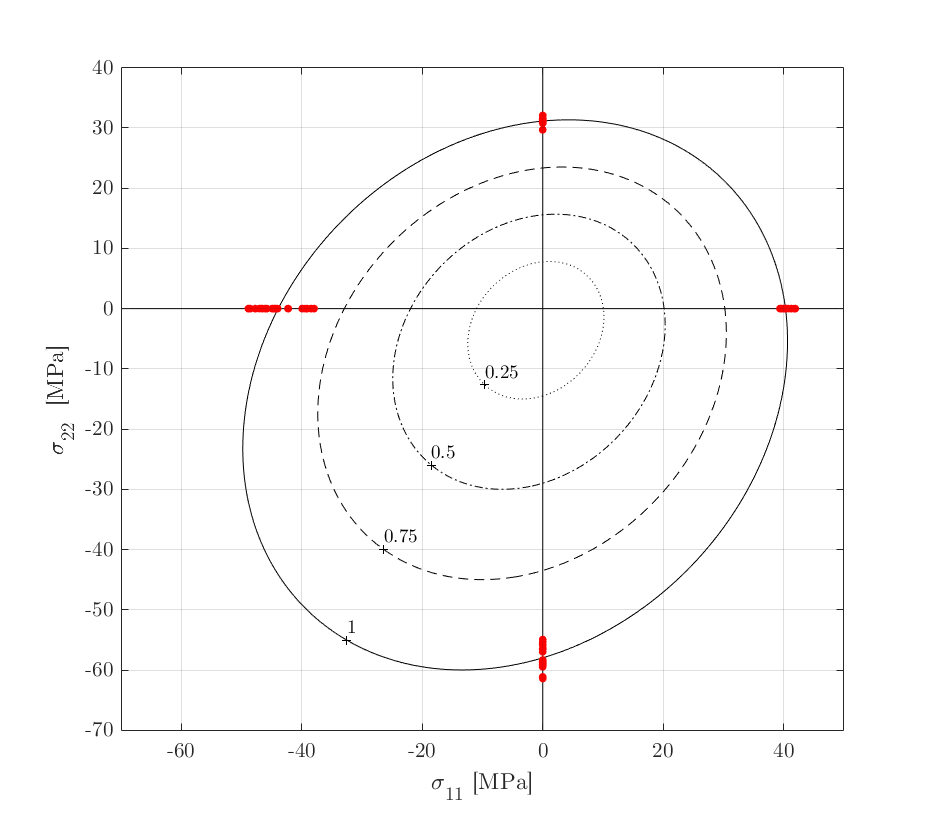
\includegraphics[width=\linewidth, keepaspectratio]{11_22plane}
	\captionsetup{justification=centering} %long caption
	\caption[failure envelope in the $\sigma_{11}$-$\sigma_{22}$ plane]{$\sigma_{11}$-$\sigma_{22}$ plane including data for reference.} \label{fig:1122plane}
\end{figure}

\pagebreak

Using the results from combined loading tests plotted in the $11-12$ and $22-12$ planes allows visualization of the transverse-axial stress interactions. Beginning with the $11-12$ plane, it can be seen that the calculated interaction slope $\mu^{1112}$ equals $5.2\times 10^{-3}$, a value that's practically zero. Using this parameter, the failure surface shown in Figure \ref{fig:1112plane} can be obtained. A dashed line representing $\mu^{1112}$ is added for reference. The $22-12$ plane by comparison reveals a considerable slope. It can be seen through the use of combined loads that there is a slight decrease in the shear strength of the specimens when a tensile load is applied in the $2-2$ direction. A slope of -0.2 was obtained for $\mu^{2212}$. Figure \ref{fig:2212plane} shows the resulting surface with the data and a line with a slope of -0.2 overlaid for reference.

\pagebreak

\begin{figure}[h]
	\center
	\subfloat[failure envelope in the $\sigma_{11}$-$\tau_{12}$ plane\label{fig:1112plane}]{%
		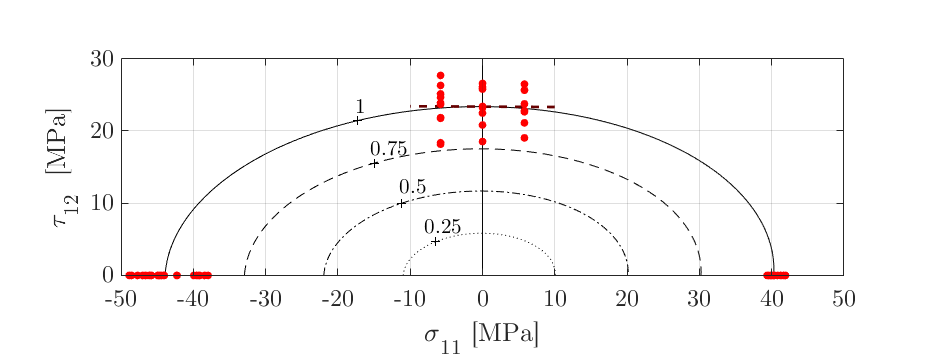
\includegraphics[width=0.9\linewidth, keepaspectratio]{11_12plane}
	}
	\linebreak
	\subfloat[failure envelope in the $\sigma_{22}$-$\tau_{12}$ plane\label{fig:2212plane}]{%
		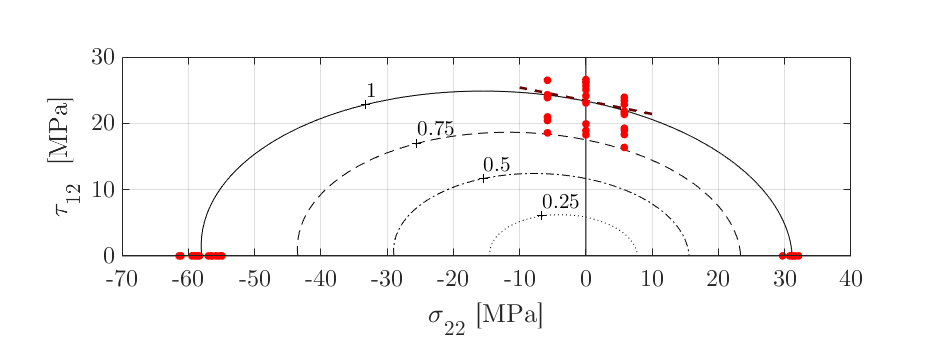
\includegraphics[width=0.9\linewidth, keepaspectratio]{22_12plane}
	}
	\caption{Comparison of interaction slopes in the axial-transverse stress planes} \label{fig:SSIcomp}
\end{figure}

The validity of the envelope was tested by Mazzei Capote  \emph{et al.} \cite{MazzeiJCompSci} in 2019. In this study, the failure function was used to estimate the failure stress of mechanical coupons loaded under tension, with a variety of raster angles being used to generate a complex loading state in the local coordinate system. Results indicated the failure prediction boundary was within 5 to 10\% of the real value. Results are summarized in Figure \ref{fig:jcompscir}, where the average of 5 mechanical tests per raster angle is represented in a dot, and the SSIC predicted failure stress is shown in a bright red line. These are compared to simpler FC, such as the maximum stress criteria in the $\sigma_{11}$, $\sigma_{22}$, and $\tau_{12}$ directions, labeled M1-1, M2-2, and M1-2 respectively. 

\begin{figure}[!htbp]
	\center
	\subfloat[Loading \label{fig:complload}]{%
		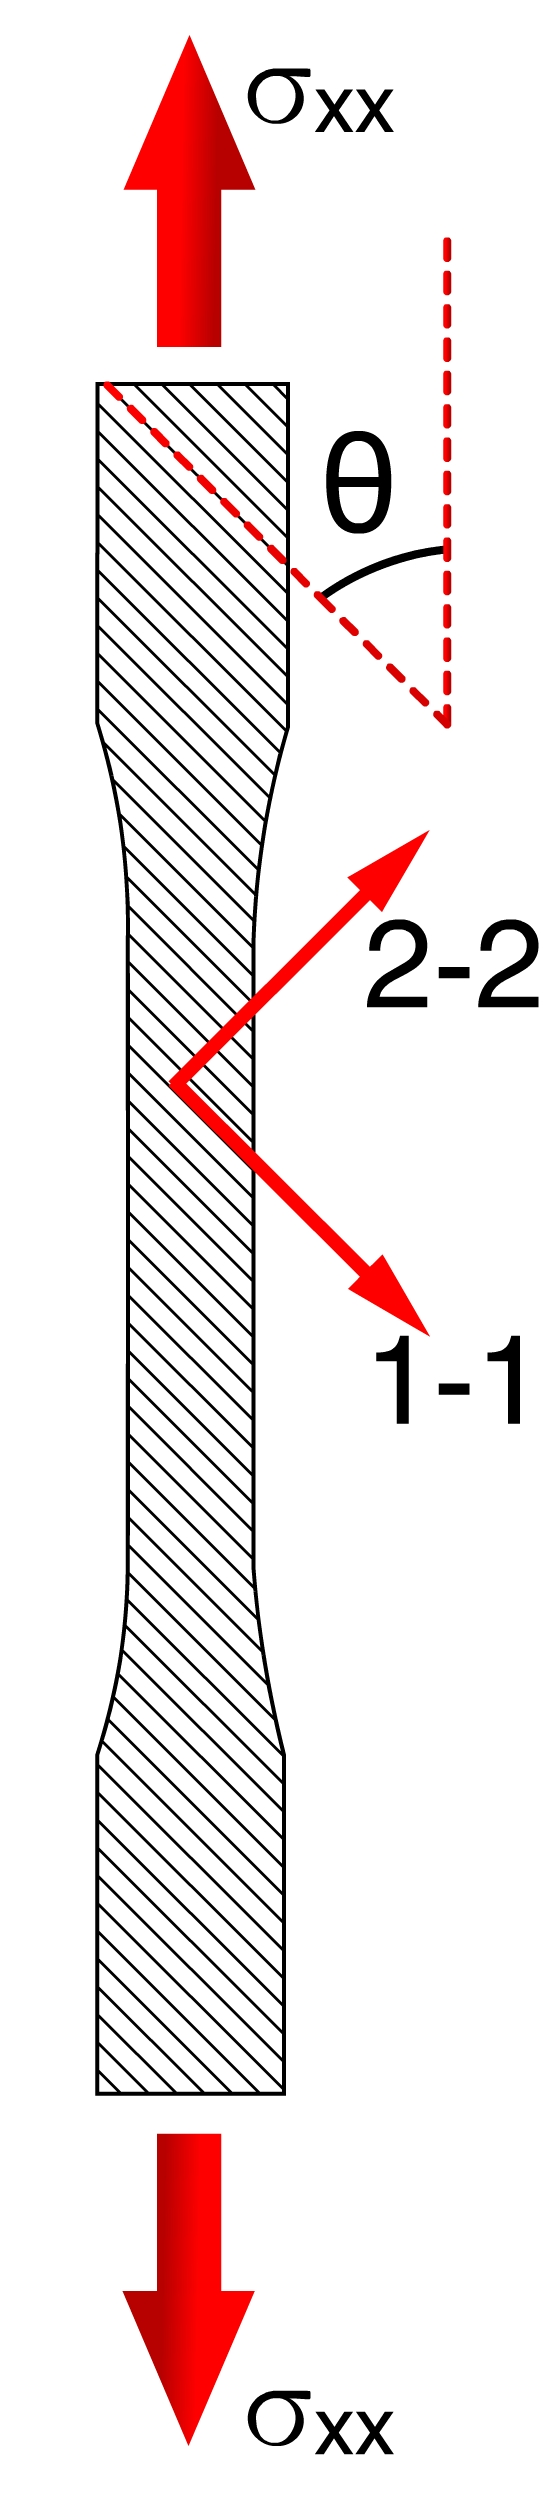
\includegraphics[height=9cm, keepaspectratio]{compl_load.jpg}
	}
	\hfill
	\subfloat[Comparison of data and failure prediction using various FC\label{fig:compsci}]{%
		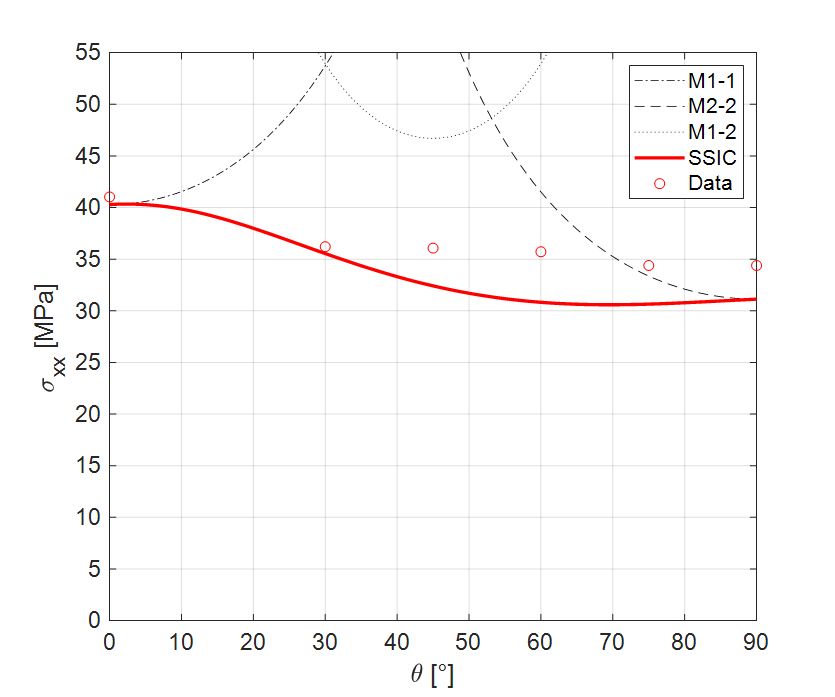
\includegraphics[height=9cm, keepaspectratio]{FC_comp.png}
	}
	\caption{Results from \cite{MazzeiJCompSci}} \label{fig:jcompscir}
\end{figure} 

While the use of FC in AM is promising, its adoption has been limited in scope. Part of the problem lies in the large number of mechanical tests required to achieve a trustworthy failure envelope, as well as the requirement of specialized equipment \textendash~such as a variety of mechanical testing devices, as well as specialized printing solutions as seen in the FFF failure envelope. Section \ref{sec:ml} outlines  machine learning methods, that can be used to predict the mechanical response of FFF parts based on process parameters. Some, if not all of the concepts explored could easily be extrapolated to other AM techniques. It should be noted that the two methods are not mutually exclusive. A combination of both FC and machine learning predictive methods can potentially lead to higher adoption rates of AM in industrial scenarios where the final desired application involves complex mechanical loads upon the finished part.

The use of AM technologies to produce small batches of highly customized, complex parts, in a reduced development cycle results extremely attractive. While constructing failure envelopes can help overcome the wariness of industrial segments to design end-user parts, this resource is still not easy to implement, requiring a large number of mechanical tests and specialized equipment to properly map the failure behavior of a particular material. Additional complexity stems from what was shown in Chapter \ref{ch:oocrit}: processing the same material under related AM technologies yields completely different failure envelopes, implying that no generalizations should be made, and each material-process pairing needs to be studied on a case-by-case basis. In general, for AM parts to be adopted, engineers have to be able to confidently assess the probability of part failure under particular loading conditions, predict the expected mechanical properties of AM parts, and understand the underlying physics of the process. None of these conditions are completely met at the time of this work.

This work aims to provide the tools required to understand and predict mechanical performance of parts manufactured through FFF through the use of Machine Learning technologies (ML), based on process variables measured during a print using an FFF printer modified with sensors. Additionally, some, if not all of the procedures developed in this work could be extrapolated to other AM techniques.

\section{Machine Learning Techniques} \label{sec:ml}

The relationship between printing conditions and final mechanical response of FFF parts is not completely understood, and the physics that govern the process appear to be complex. Multiple attempts have been made to model the physics of the melting process that occurs inside the nozzle, each with their own set of assumptions that do not seem to fully grasp the nature of the small scale extrusion occurring with the FFF technology \cite{ColonQuintana2020}. While it is understood that processing parameters have an impact on the final dimensions of the extruded polymer beads, there is a clear disconnect between how it relates to the process physics \cite{Koch2017}. However, this constitutes an interesting case for development of a Machine Learning (ML) solution, which excel in cases where the inputs and outcomes of a particular phenomena or task are known, but connecting the two through an explicit set of rules or relationships can result extremely complex and time consuming \cite{Chollet2018}. In this manner, ML models are \emph{trained}, as opposed to explicitly defined, as illustrated in Figure \ref{fig:MLvsP}, where the differences between ML and traditional programming philosophies are compared. 

\begin{figure}[!htbp]
	\center
	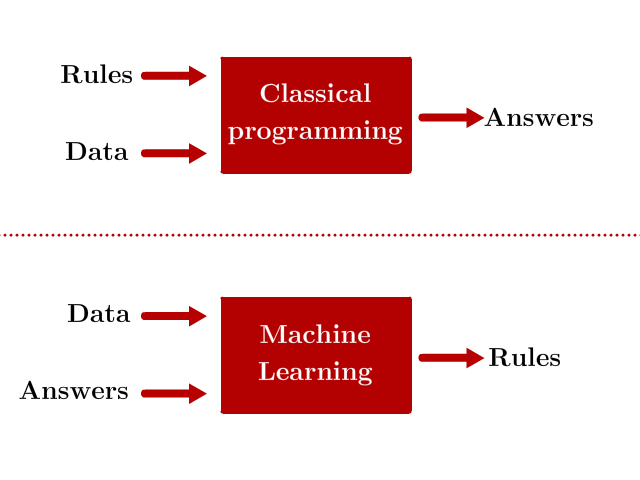
\includegraphics[height=6cm]{ML}
	\caption{Differences between traditional programming and machine learning. \cite{Chollet2018}} \label{fig:MLvsP}
\end{figure}

The potential to apply ML solutions in the field of AM has been noted by several authors \cite{Razvi2019,Meng2020}. Example cases include design-recommendation systems, topology optimization solutions, tolerancing and manufacturability assessment, and material classification and selection \cite{Razvi2019}. Machine learning algorithms are varied, and a summary of how they have been recently applied to AM can be seen in Figure \ref{fig:supL}.

\begin{figure}[!htbp]
	\center
	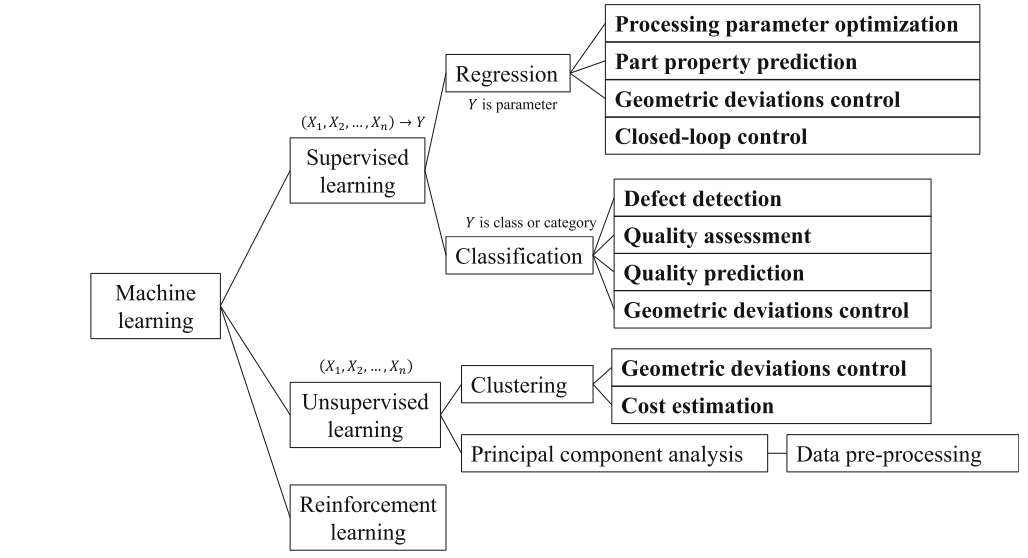
\includegraphics[height=7.5cm]{SL}
	\caption{Taxonomy of ML applications in AM \cite{Meng2020}} \label{fig:supL}
\end{figure}

% Start here
Given the factors outlined this far, the fundamental goal of this research is to predict FFF part mechanical performance by finding relations between processing conditions and strength through the use of sensors and machine learning. The success of this project would allow design engineers to confidently assess if a part manufactured through FFF will meet the mechanical requirements imposed by its intended application. This work proposes developing and using a modified printer with force and print speed sensors, as well as mechanical testing and $\mu$CT scans to generate data that can be used to train a predictive tool based on ML. This tool can then be used to predict final mechanical properties of the part based on the data generated during the print. 

%______________________________________________________________________________________
% Nomenclature introduced in this chapter:
\nomenclature[A]{SLA}{Stereolithography}% 
\nomenclature[A]{SLS}{Selective Laser Sintering}%
\nomenclature[A]{$\mu$CT}{Micro Computer Tomography}%
\nomenclature[A]{SSIC}{Stress-Stress Interaction Criterion}% 
\nomenclature[A]{GKC}{Gol'denblat-Kopnov Criterion}% 
\nomenclature[A]{MJF}{Multi-Jet Fusion}% 
\nomenclature[A]{PBF}{Powder Bed Fusion}% 
\nomenclature[A]{SSIC}{Stress-Stress Interaction Criterion}% 
\nomenclature[A]{GKC}{Gol'denblat-Kopnov Criterion}% 
\nomenclature[A]{MJF}{Multi-Jet Fusion}% 
\nomenclature[A]{PBF}{Powder Bed Fusion}% 
\nomenclature[A]{ML}{Machine Learning}% 
\nomenclature[A]{SVM}{Support Vector Machines}%
\nomenclature[A]{NN}{Neural Network}%
\nomenclature[A]{MSE}{Mean Square Error}%
\nomenclature[A]{MAE}{Mean Absolute Error}%

% Symbols introduced in this chapter:
\nomenclature[S]{$\sigma$}{Axial stress \nomunit{$MPa$}}
\nomenclature[S]{$\tau$}{Shear stress \nomunit{$MPa$}}
\nomenclature[S]{$\sigma_{11}$}{Axial stress in the 1-1 direction \nomunit{$MPa$}}
\nomenclature[S]{$\sigma_{22}$}{Axial stress in the 2-2 direction \nomunit{$MPa$}}
\nomenclature[S]{$\sigma_{33}$}{Axial stress in the 3-3 direction \nomunit{$MPa$}}
\nomenclature[S]{$\tau_{12}$}{Shear stress in the 1-2 plane \nomunit{$MPa$}}
\nomenclature[S]{$\tau_{13}$}{Shear stress in the 1-3 plane \nomunit{$MPa$}}
\nomenclature[S]{$\tau_{23}$}{Shear stress in the 2-3 plane \nomunit{$MPa$}}
\nomenclature[S]{$X_t$}{Tensile strength in the 1-1 direction \nomunit{$MPa$}}
\nomenclature[S]{$X_c$}{Compressive strength in the 1-1 direction \nomunit{$MPa$}}
\nomenclature[S]{$Y_t$}{Tensile strength in the 2-2 direction \nomunit{$MPa$}}
\nomenclature[S]{$Y_c$}{Compressive strength in the 2-2 direction \nomunit{$MPa$}}
\nomenclature[S]{$S$}{Shear strength in the 1-2 plane \nomunit{$MPa$}}
\nomenclature[S]{$S_{45p}$}{Positive shear strength for 45$^\circ$ specimen \nomunit{$MPa$}}
\nomenclature[S]{$S_{45n}$}{Negative shear strength for 45$^\circ$ specimen \nomunit{$MPa$}}
\nomenclature[S]{$\mu^{1112}$}{SSIC parameter- slope at pure shear failure in the $\sigma_{11}$ - $\tau_{12}$ plane \nomunit{$-$}}
\nomenclature[S]{$\mu^{2212}$}{SSIC parameter- slope at pure shear failure in the $\sigma_{22}$ - $\tau_{12}$ plane \nomunit{$-$}}
\nomenclature[S]{$X_t$}{Tensile strength in the 1-1 direction \nomunit{$MPa$}}
\nomenclature[S]{$X_c$}{Compressive strength in the 1-1 direction \nomunit{$MPa$}}
\nomenclature[S]{$Y_t$}{Tensile strength in the 2-2 direction \nomunit{$MPa$}}
\nomenclature[S]{$Y_c$}{Compressive strength in the 2-2 direction \nomunit{$MPa$}}
\nomenclature[S]{$S$}{Shear strength in the 1-2 plane \nomunit{$MPa$}}
\nomenclature[S]{$S_{45p}$}{Positive shear strength for 45$^\circ$ specimen \nomunit{$MPa$}}
\nomenclature[S]{$S_{45n}$}{Negative shear strength for 45$^\circ$ specimen \nomunit{$MPa$}}
\nomenclature[S]{$\mu^{1112}$}{SSIC parameter- slope at pure shear failure in the $\sigma_{11}$ - $\tau_{12}$ plane \nomunit{$-$}}
\nomenclature[S]{$\mu^{2212}$}{SSIC parameter- slope at pure shear failure in the $\sigma_{22}$ - $\tau_{12}$ plane \nomunit{$-$}}
\end{document}
                %% oocriterion.tex
\documentclass[main.tex]{subfiles}
\begin{document}
\chapter{Previous work} \label{ch:oocrit}


The SSIC offers a way of capturing in a more accurate manner the different failure modes of parts produced through AM technologies. As an example, the model has been successfully implemented by Obst \emph{et al.} in 2018 for SLS manufactured parts produced with PA12 \cite{Obst2018, Obst2017}. Their results show how the model was able to capture the $\tau_{12}$-$\sigma_{22}$ and $\sigma_{11}$-$\sigma_{22}$ interactions. The failure surface obtained, shown in Figure \ref{fig:OOCSLS}, was able to capture the interactions between certain axial and transverse stresses. However, due to the limitations of the SLS process, it was not possible to measure the interaction slope between the $\tau_{12}$ and $\sigma_{11}$ directions.

\begin{figure}[h]
	\center
	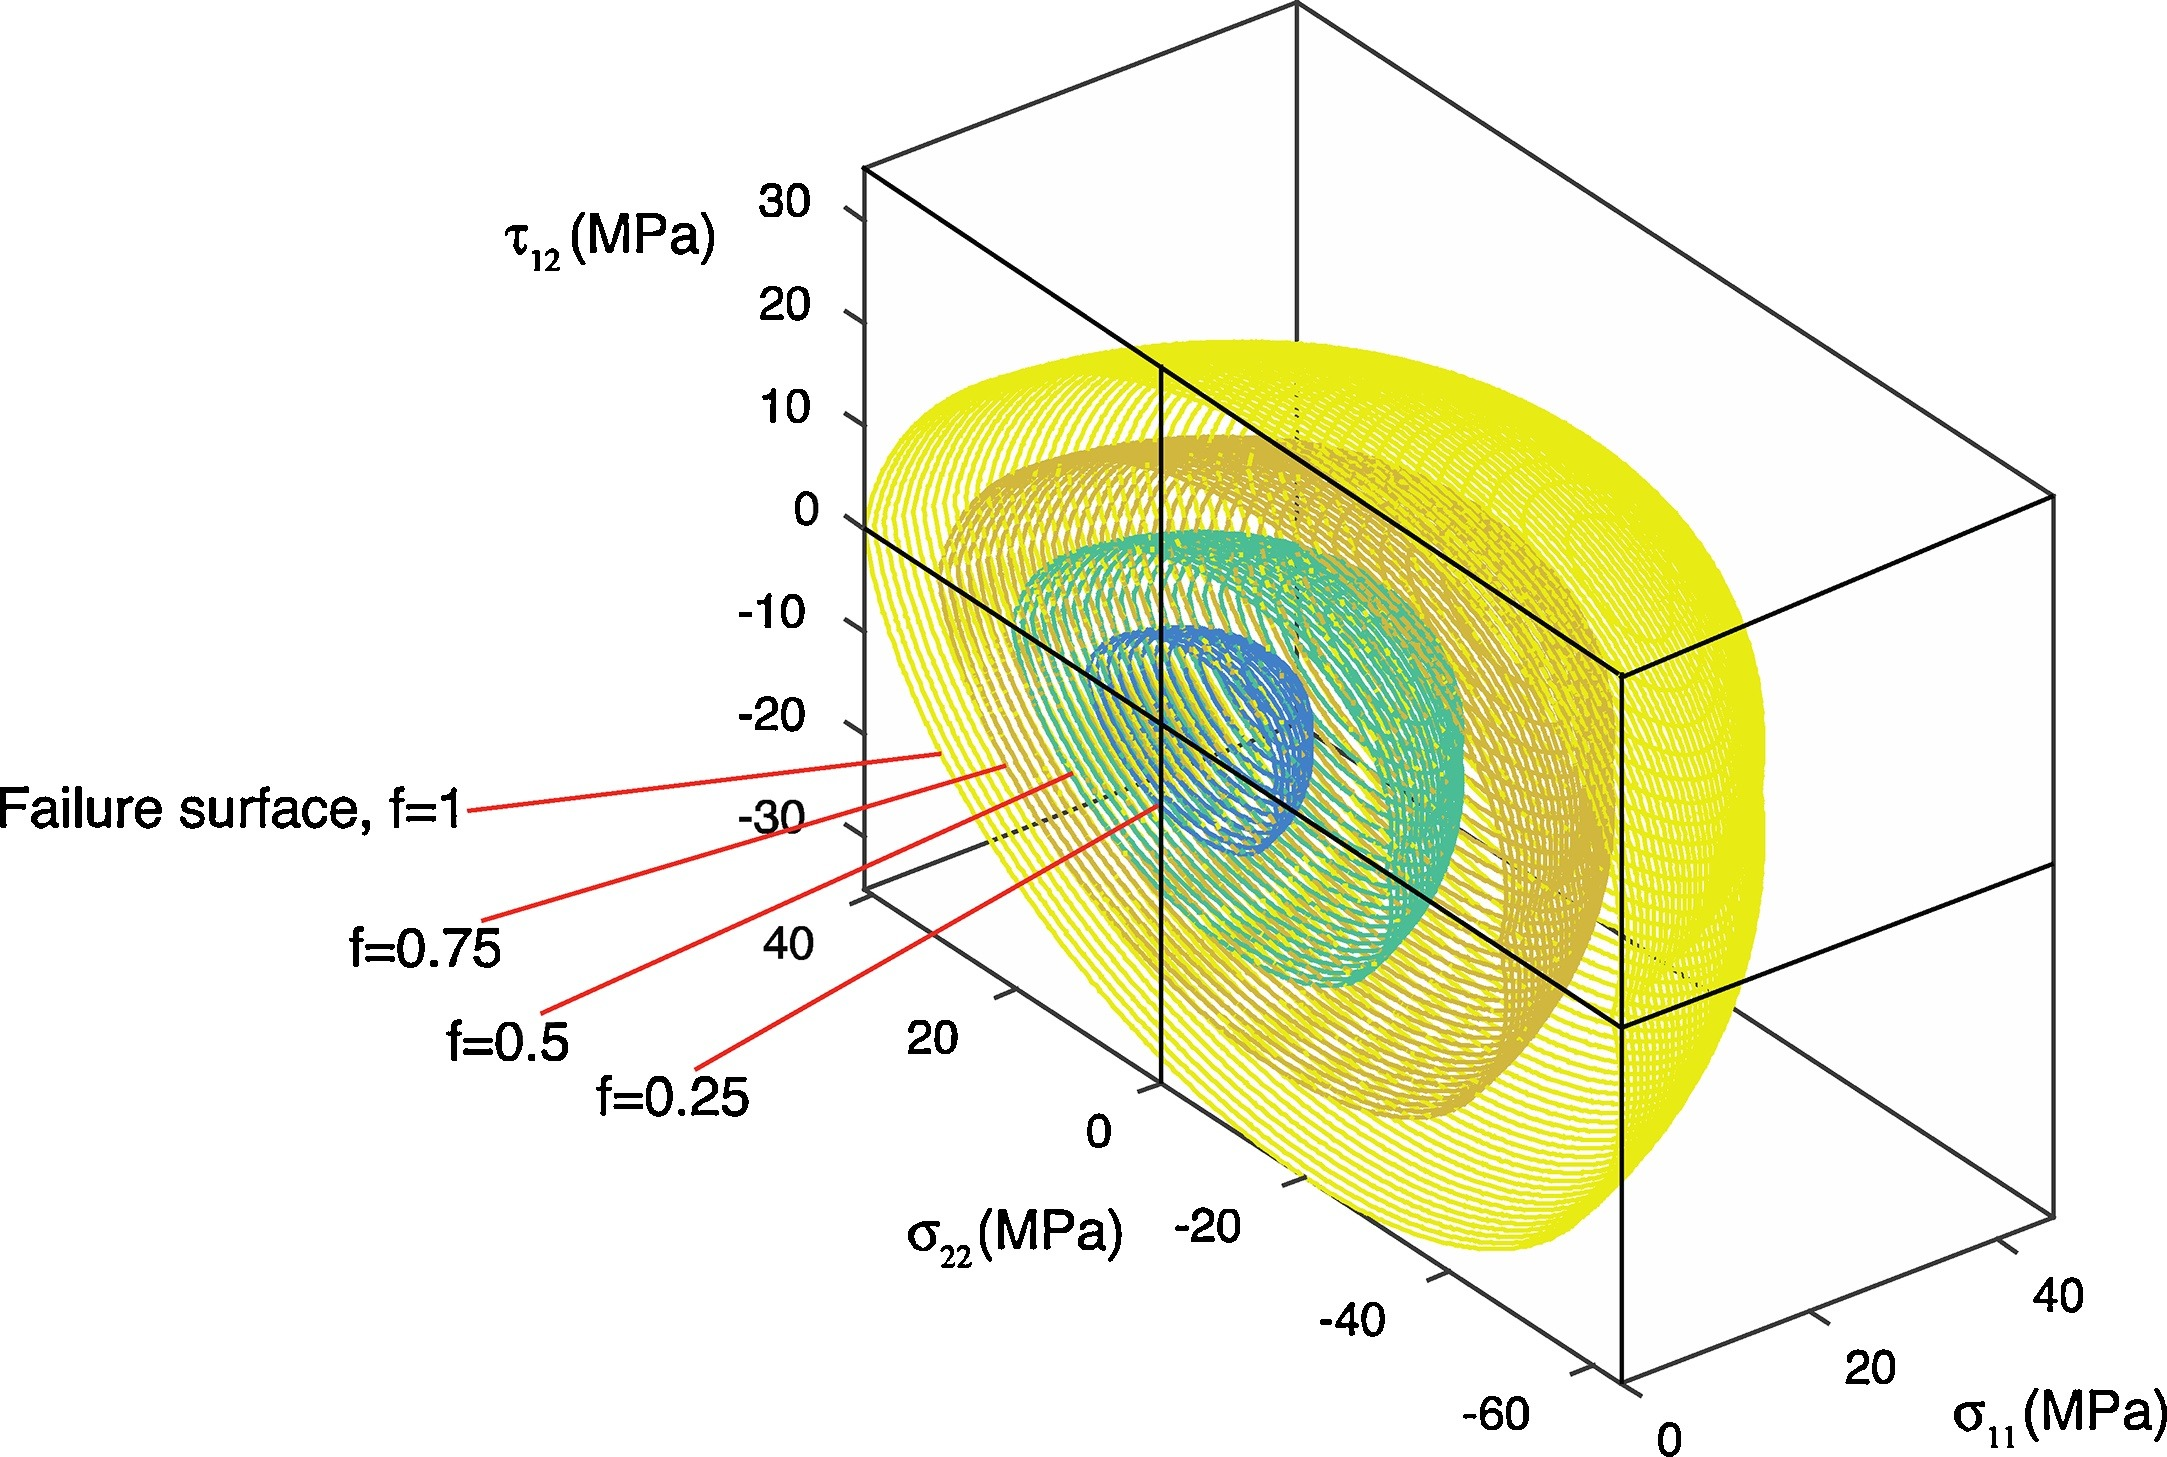
\includegraphics[height=6cm]{Obst_SLS}
	\caption{Failure surface for SLS developed through the SSIC \cite{Obst2018}} \label{fig:OOCSLS}
\end{figure}

Recent unpublished work by Osswald \emph{et al.} \cite{Osswald2020} generated a failure envelope for Multi-Jet Fusion (MJF) parts produced using PA12, and compared it to the surface obtained by Obst \emph{et al.} \cite{Obst2018}. Results indicate that, while both techniques are based on Powder Based Fusion (PBF) and use the same material, the envelopes for each AM technology were distinct, serving as proof that these technologies are not as comparable under complex loading conditions as previously assumed. The transverse-axial interaction for the MJF case was significantly less pronounced than for SLS, further reinforcing that each AM technique needs to be studied in a case-by-case basis in terms of mechanical failure characterization. 

\begin{figure}[!htbp]
	\center
	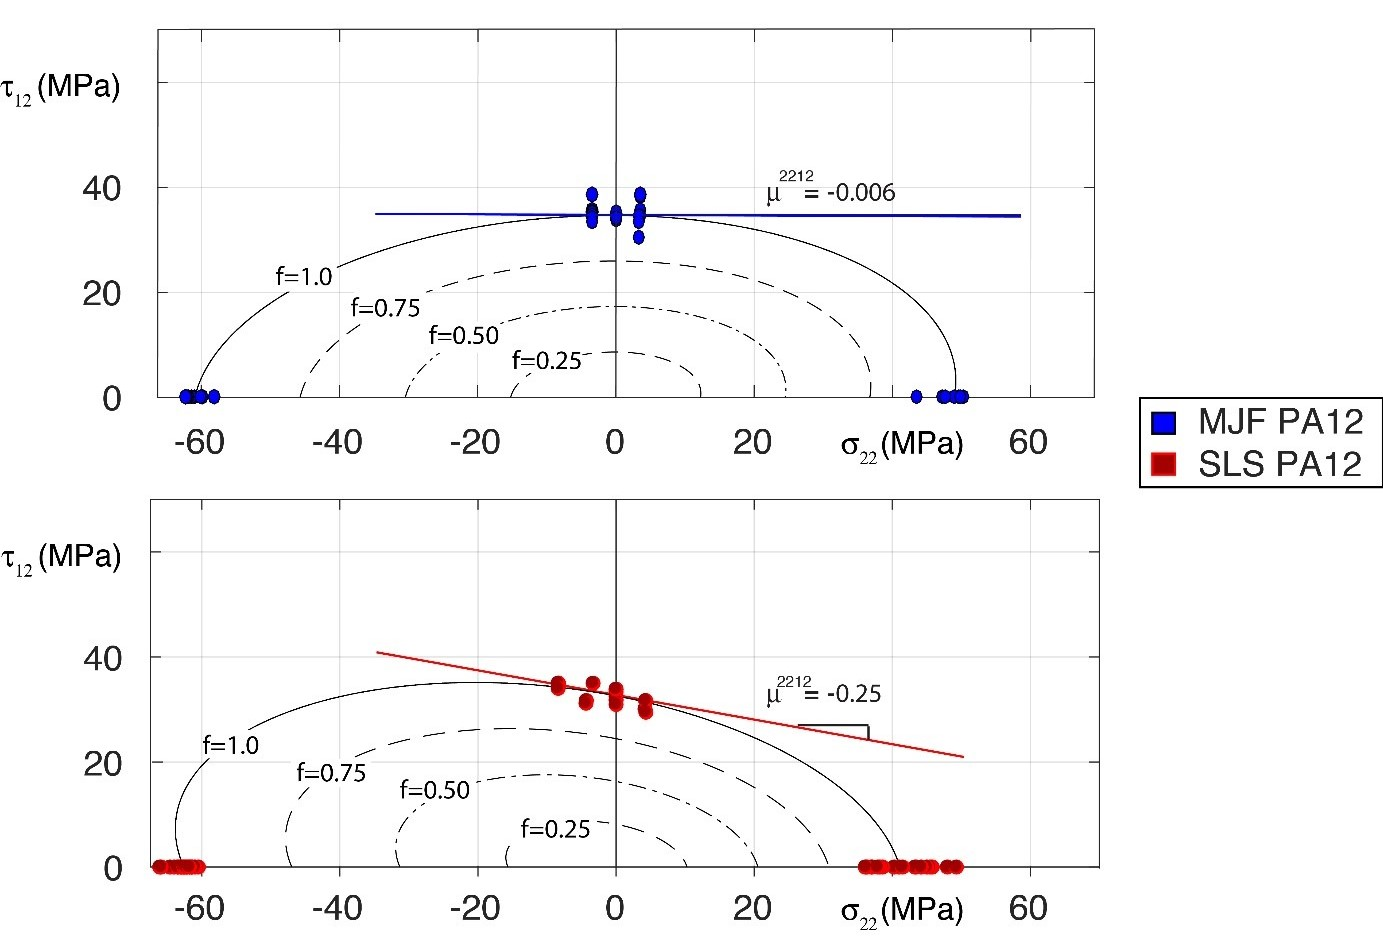
\includegraphics[height=10cm]{pbfcomp}
	\caption{Comparison of the $\sigma_{22} - \tau_{12}$ interaction for SLS and MJF PA12 parts \cite{Osswald2020}} \label{fig:pbfcomp}
\end{figure}

\section{Development of SSIC envelope for FFF parts}\label{sec:SSICFFF}

In 2019, Mazzei Capote \emph{et al.} \cite{MazzeiCapote2019} developed a failure envelope for FFF parts produced using a customized ABS filament produced in-house. Specimens were produced using either a commercially available desktop FFF printer (Lulzbot TAZ5, USA), or a customized 6-axis robotic printing solution whenever the bead orientation was hard to achieve using a \emph{2.5-D} machine. The robotic printer was based on a 6-axis robot (ABB IRB-120, Switzerland) and fitted with a stationary printhead mounted on an aluminum frame, chosen to be the same extruder from the traditional printer (LulzBot TAZ Single Extruder Tool Head v2, 0.5 mm nozzle, USA) to minimize machine influence on the results \cite{VanHulle2017}. The final surface obtained showed significant stress interactions in certain directions. Starting with the $\sigma_{11}$-$\sigma_{22}$ plane, it can be seen that the failure envelope has a slight tilt. Refer to Figure~\ref{fig:1122plane} for a graph showing the calculated failure envelope, including the experimental data for reference. This tilt is evidence of an interaction between the transverse and longitudinal stresses. The conclusion is that FFF parts produced with the print parameters used in the study should show strengthening when loaded bi-axially in compression.

\begin{figure}[h]
	\center
	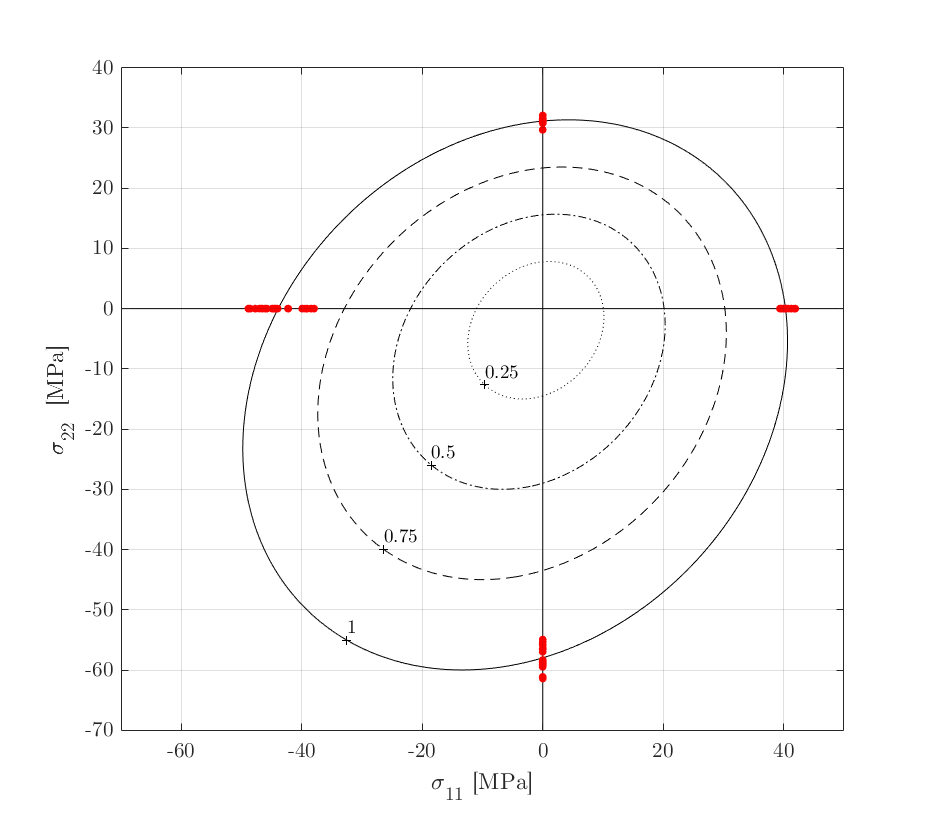
\includegraphics[width=\linewidth, keepaspectratio]{11_22plane}
	\captionsetup{justification=centering} %long caption
	\caption[failure envelope in the $\sigma_{11}$-$\sigma_{22}$ plane]{$\sigma_{11}$-$\sigma_{22}$ plane including data for reference.} \label{fig:1122plane}
\end{figure}

\pagebreak

Using the results from combined loading tests plotted in the $11-12$ and $22-12$ planes allows visualization of the transverse-axial stress interactions. Beginning with the $11-12$ plane, it can be seen that the calculated interaction slope $\mu^{1112}$ equals $5.2\times 10^{-3}$, a value that's practically zero. Using this parameter, the failure surface shown in Figure \ref{fig:1112plane} can be obtained. A dashed line representing $\mu^{1112}$ is added for reference. The $22-12$ plane by comparison reveals a considerable slope. It can be seen through the use of combined loads that there is a slight decrease in the shear strength of the specimens when a tensile load is applied in the $2-2$ direction. A slope of -0.2 was obtained for $\mu^{2212}$. Figure \ref{fig:2212plane} shows the resulting surface with the data and a line with a slope of -0.2 overlaid for reference.

\pagebreak

\begin{figure}[h]
	\center
	\subfloat[failure envelope in the $\sigma_{11}$-$\tau_{12}$ plane\label{fig:1112plane}]{%
		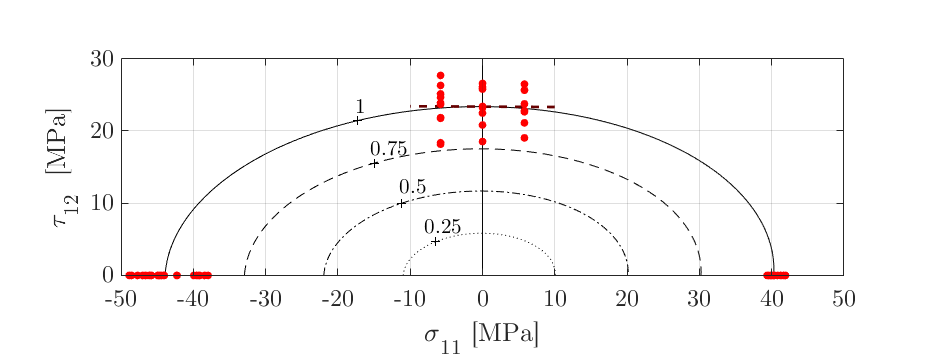
\includegraphics[width=0.9\linewidth, keepaspectratio]{11_12plane}
	}
	\linebreak
	\subfloat[failure envelope in the $\sigma_{22}$-$\tau_{12}$ plane\label{fig:2212plane}]{%
		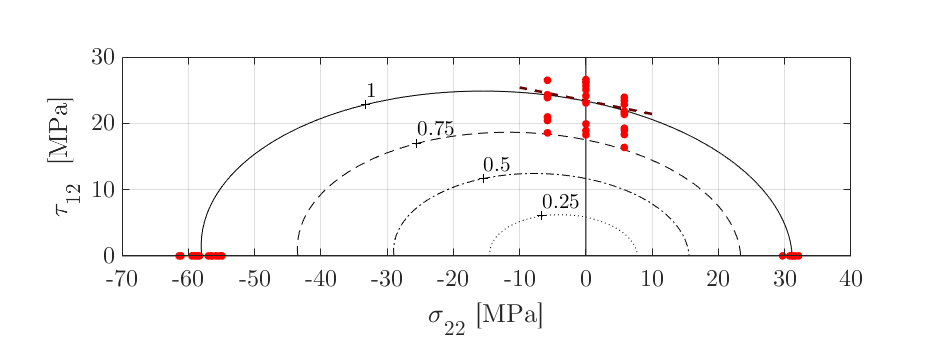
\includegraphics[width=0.9\linewidth, keepaspectratio]{22_12plane}
	}
	\caption{Comparison of interaction slopes in the axial-transverse stress planes} \label{fig:SSIcomp}
\end{figure}

\section{Validation of the FFF Failure envelope}\label{sec:FFFval}

The validity of the envelope described in Section \ref{sec:SSICFFF} was tested by Mazzei Capote  \emph{et al.} \cite{MazzeiJCompSci} in 2019. In this study, the failure function was used to estimate the failure stress of mechanical coupons loaded under tension, with a variety of raster angles being used to generate a complex loading state in the local coordinate system. Results indicated the failure prediction boundary was within 5 to 10\% of the real value. Results are summarized in Figure \ref{fig:jcompscir}, where the average of 5 mechanical tests per raster angle is represented in a dot, and the SSIC predicted failure stress is shown in a bright red line. These are compared to simpler FC, such as the maximum stress criteria in the $\sigma_{11}$, $\sigma_{22}$, and $\tau_{12}$ directions, labeled M1-1, M2-2, and M1-2 respectively. 

\begin{figure}[!htbp]
	\center
	\subfloat[Loading \label{fig:complload}]{%
		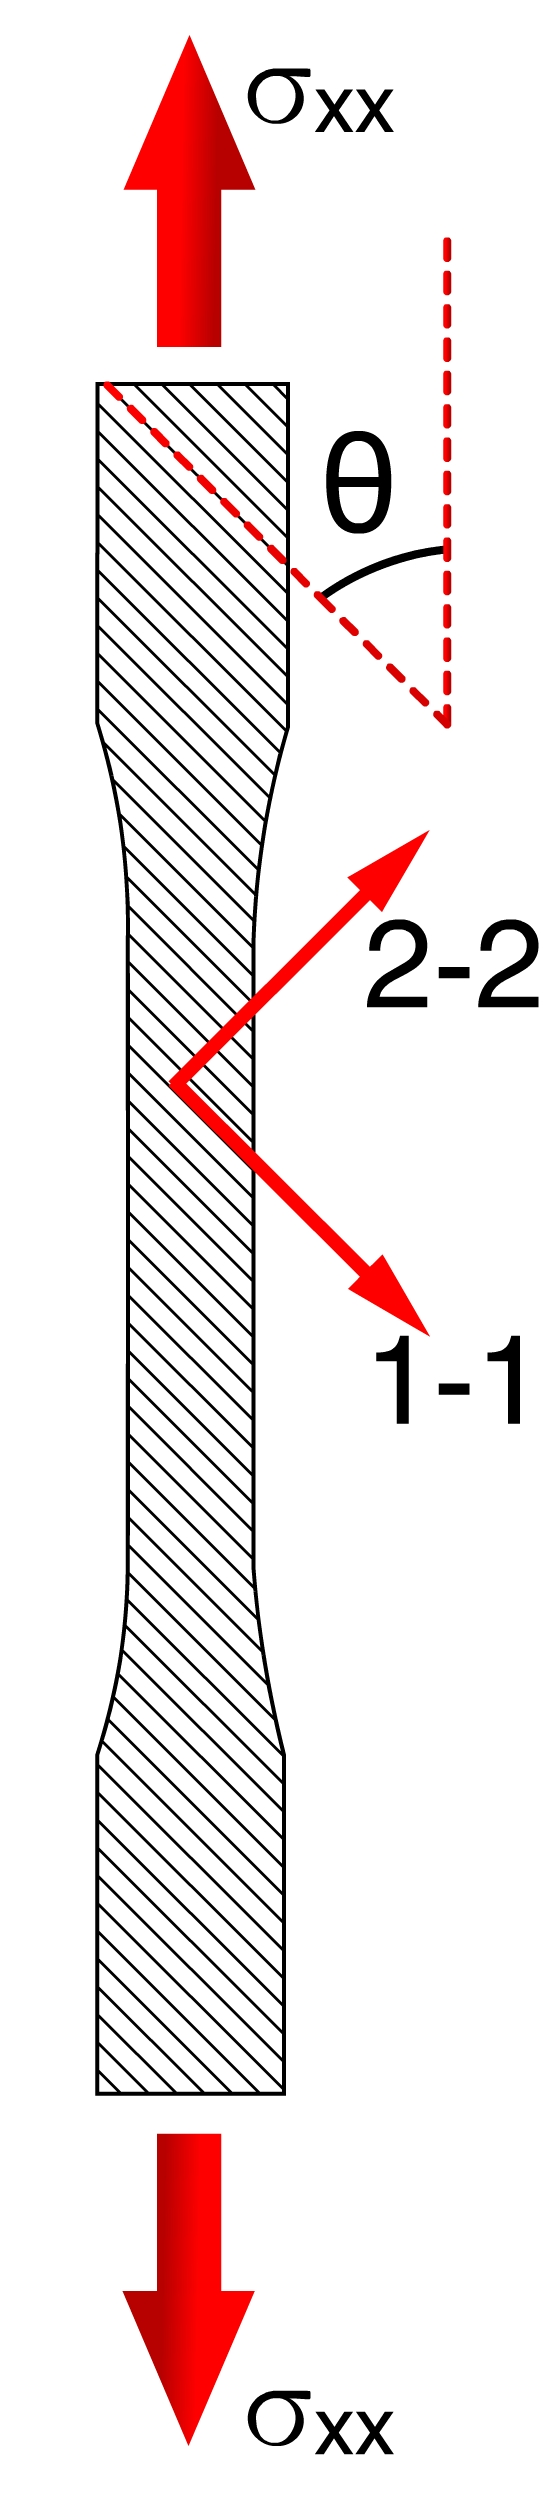
\includegraphics[height=9cm, keepaspectratio]{compl_load.jpg}
	}
	\hfill
	\subfloat[Comparison of data and failure prediction using various FC\label{fig:compsci}]{%
		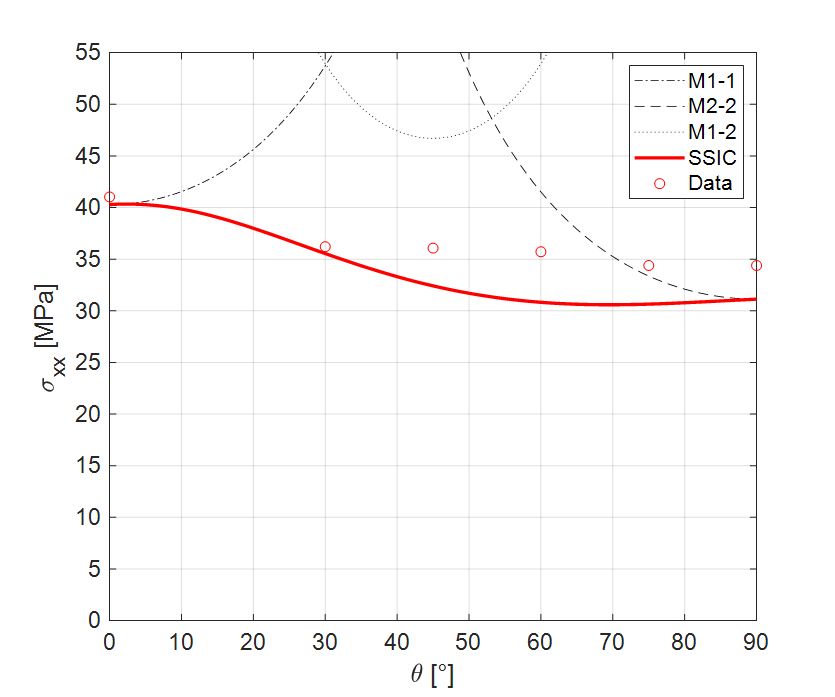
\includegraphics[height=9cm, keepaspectratio]{FC_comp.png}
	}
	\caption{Results from \cite{MazzeiJCompSci}} \label{fig:jcompscir}
\end{figure} 


While the use of FC in AM is promising, its adoption has been limited in scope. Part of the problem lies in the large number of mechanical tests required to achieve a trustworthy failure envelope, as well as the requirement of specialized equipment \textendash~such as a variety of mechanical testing devices, as well as specialized printing solutions as seen in the FFF failure envelope. Chapter \ref{ch:proposal} outlines proposed work aimed at predicting the mechanical response of FFF parts using machine learning methods. Some, if not all of the concepts explored could easily be extrapolated to other AM techniques. It should be noted that the two methods are not mutually exclusive. A combination of both FC and machine learning predictive methods can hopefully lead to a higher adoption rates of AM in industrial scenarios where the final desired application involves complex mechanical loads upon the finished part. 

% Nomenclature introduced in this chapter:
\nomenclature[A]{SSIC}{Stress-Stress Interaction Criterion}% 
\nomenclature[A]{GKC}{Gol'denblat-Kopnov Criterion}% 
\nomenclature[A]{MJF}{Multi-Jet Fusion}% 
\nomenclature[A]{PBF}{Powder Bed Fusion}% 

% Symbols introduced in this chapter:
\nomenclature[S]{$X_t$}{Tensile strength in the 1-1 direction \nomunit{$MPa$}}
\nomenclature[S]{$X_c$}{Compressive strength in the 1-1 direction \nomunit{$MPa$}}
\nomenclature[S]{$Y_t$}{Tensile strength in the 2-2 direction \nomunit{$MPa$}}
\nomenclature[S]{$Y_c$}{Compressive strength in the 2-2 direction \nomunit{$MPa$}}
\nomenclature[S]{$S$}{Shear strength in the 1-2 plane \nomunit{$MPa$}}
\nomenclature[S]{$S_{45p}$}{Positive shear strength for 45$^\circ$ specimen \nomunit{$MPa$}}
\nomenclature[S]{$S_{45n}$}{Negative shear strength for 45$^\circ$ specimen \nomunit{$MPa$}}
\nomenclature[S]{$\mu^{1112}$}{SSIC parameter- slope at pure shear failure in the $\sigma_{11}$ - $\tau_{12}$ plane \nomunit{$-$}}
\nomenclature[S]{$\mu^{2212}$}{SSIC parameter- slope at pure shear failure in the $\sigma_{22}$ - $\tau_{12}$ plane \nomunit{$-$}}
\end{document}
                %% proposal.tex
\documentclass[main.tex]{subfiles}
\begin{document}
\chapter{Prediction of Mechanical Properties through Machine Learning} \label{ch:ml}

\section{Foreword} \label{sec:fw_ml}

The use of AM technologies to produce small batches of highly customized, complex parts in a reduced development cycle results extremely attractive to all industries. However, for AM parts to be fully adopted in industrial scenarios, engineers have to be able to confidently assess the structural integrity of the finished part under its intended loading conditions. This requirement is unfortunately not fully possible at the time this work was produced, partly because the mechanical properties of AM tend to be anisotropic, and partly because the relationships that exist between processing parameters, underlying physics of the process, and final mechanical part properties aren't fully comprehended. However, these obstacles present an interesting case for the application of Machine Learning (ML) techniques, where the inputs and outputs of a particular phenomenon are known, but there's a lack of explicit rules that indicate a relationship between the two. 

This work uses the Fused Filament Fabrication (FFF) process as a case study for the application of ML techniques to predict the final mechanical properties of a printed part. Experimental work involved producing a variety of tensile coupons, developed under various printing conditions, and where the filament extrusion speed, filament extrusion force, and printing temperature were measured in real time using machines fitted with in-line sensors. These specimens were then tested up to tensile failure, and the collective data of printing parameters, measured process indicators, and mechanical tests results were used to train a Neural Network capable of predicting the tensile failure stress.

In the context of this dissertation, this represents an alternative method for part failure prediction to construction and evaluation of a failure envelope. However, it should be noted that both methods are not mutually exclusive, and as will be discussed under future work, the author believes they can be combined quite well. 

\section{Introduction} \label{sec:ml_intr}

The set of printing conditions that lead to an optimal part in terms of mechanical properties aren't still fully comprehended. However, if there existed an FFF machine with in-line sensors that allowed monitoring a variety of process-variables, as well as data generated from mechanical tests and ancillary experiments, this would constitute an interesting case for development of a Machine Learning (ML) system. These excel in cases where the inputs and outcomes of a particular phenomena or task are known, but connecting the two through an explicit set of rules or relationships can result extremely complex and time consuming \cite{Chollet2018}. In this manner, ML models are \emph{trained}, as opposed to explicitly programmed, as illustrated in Figure \ref{fig:MLvsP}, where the differences between ML and traditional programming philosophies are compared. 

\begin{figure}[!htbp]
	\center
	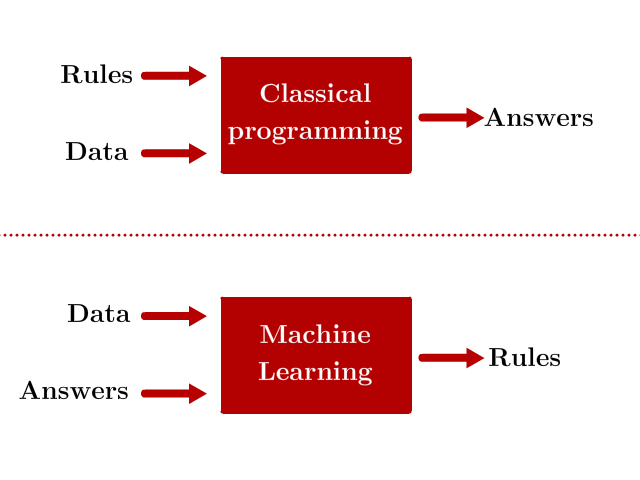
\includegraphics[height=6cm]{ML}
	\caption{Differences between traditional programming and machine learning. \cite{Chollet2018}} \label{fig:MLvsP_2}
\end{figure}

The potential to apply ML solutions in the field of AM has been noted by several authors \cite{Razvi2019,Meng2020}. Example cases include design-recommendation systems, topology optimization solutions, tolerancing and manufacturability assessment, and material classification and selection \cite{Razvi2019}. The specific algorithm applied for each case varied wildly depending on the nature of the task, but in general, Support Vector Machines (SVM) and Neural Networks (NN) appear to be the most prevalent solutions.

Given the factors outlined this far, the fundamental goal of this research is to predict FFF part mechanical performance by finding relations between processing conditions and strength through the use of sensors and machine learning. The success of this project would allow design engineers to confidently assess if a part manufactured through FFF will meet the mechanical requirements imposed by its intended application. This work proposes developing and using a modified printer with force and print speed sensors, as well as mechanical testing and $\mu$CT scans to generate data that can be used to train a predictive tool based on ML. This tool can then be used to predict final mechanical properties of the part based on the data generated during the print. This ML system would accept filament dimensions, printing temperature, filament force, filament velocity, print orientation, layer height, or any subset of these items as inputs, and produce final part porosity and/or mechanical strength in a particular load direction as outputs. These parameters were chosen based on previous work performed by Koch, Van Hulle and Rudolph \cite{Koch2017}, where the final tensile strength of FFF coupons was shown to be related to the morphology of the printed bead, which is significantly affected by processing parameters and variations in the volumetric output of the nozzle; research published by Sood \emph{et al.} \cite{Sood2012} where a NN was able to predict the compressive strength of FDM parts with an $R^2= 0.9977$ using layer thickness, raster angle, orientation, raster width, and air gap as inputs; as well as the proposed FFF melting models established by Bellini \emph{et al.} \cite{Bellini2004} and Osswald \emph{et al.} \cite{OsswaldMelting18}. The specifics of the architecture of the ML system are still under development, as it may prove useful to segment the problem into several sub-systems connected in series, in what is called a machine learning \emph{pipeline} \cite{Geron2019}. However, given the specifics of the task, one can conclude that the system will involve supervised learning applied to a regression problem, given that all the inputs to the system will consist of pre-selected attributes, and the mechanical response and/or porosity of a printed part can be treated as a target value the ML system has to be able to predict \cite{Mohammed2017, Meng2020}.


\section{Experimental Methods} \label{sec:ml_meth}

\subsection{Feature Selection and Engineering} \label{ssec:ml_fs}
\begin{figure}[!htbp]
	\center
	\includegraphics[height=7cm]{forcesetup}
	\caption{Schematic of modified FFF printer with sensors} \label{fig:shakira}
\end{figure}

\begin{figure}[!htbp]
	\center
	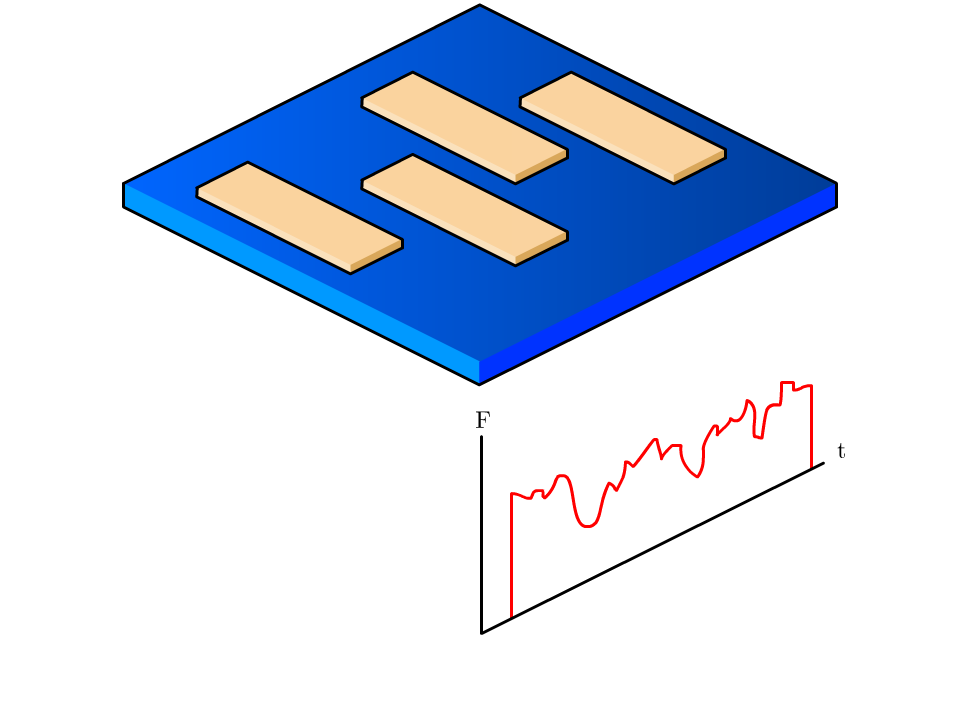
\includegraphics[height=8cm]{coupon_print_diagram}
	\caption{Schematic of print experiment} \label{fig:print_dia}
\end{figure}

\begin{figure}[!htbp]
	\center
	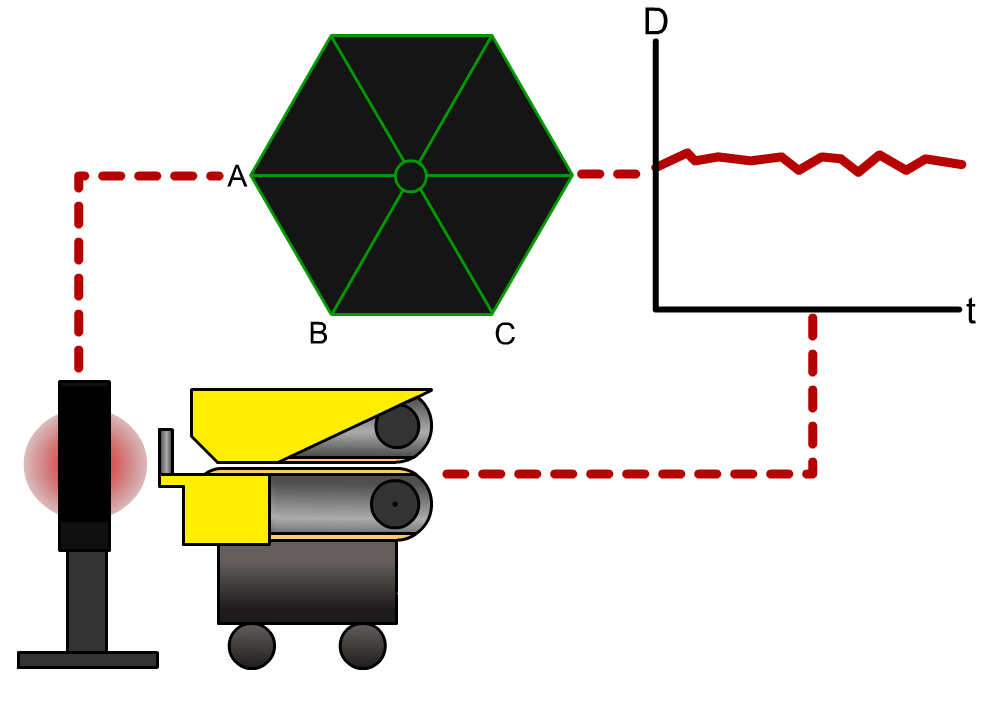
\includegraphics[width=0.6\linewidth]{filament_measurement}
	\caption{Filament geometry information, acquired through a laser micrometer } \label{fig:FD}
\end{figure}

\begin{figure}[h]
	\center
	\subfloat[Effect of diameter on measured filament speed \label{fig:D_sp}]{%
		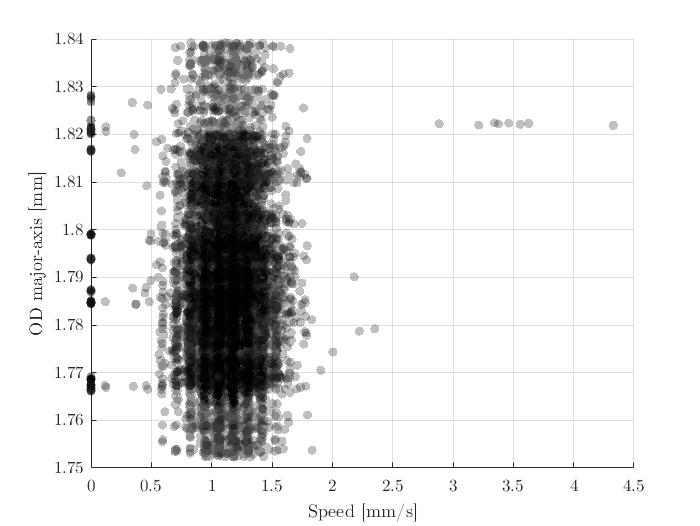
\includegraphics[width=0.8\linewidth, keepaspectratio]{speed-OD}
	}
	\linebreak
	\subfloat[Effect of diameter on measured filament force \label{fig:D_f}]{%
		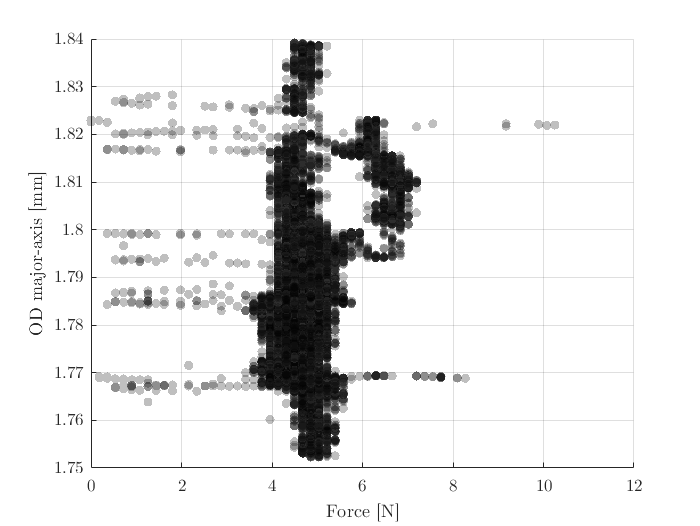
\includegraphics[width=0.8\linewidth, keepaspectratio]{force-OD}
	}
	\caption{Effect of diameter on filament force and speed} \label{fig:dia_f_sp}
\end{figure}

\begin{figure}[h]
	\center
	\subfloat[Effect of ovality on measured filament speed \label{fig:O_sp}]{%
		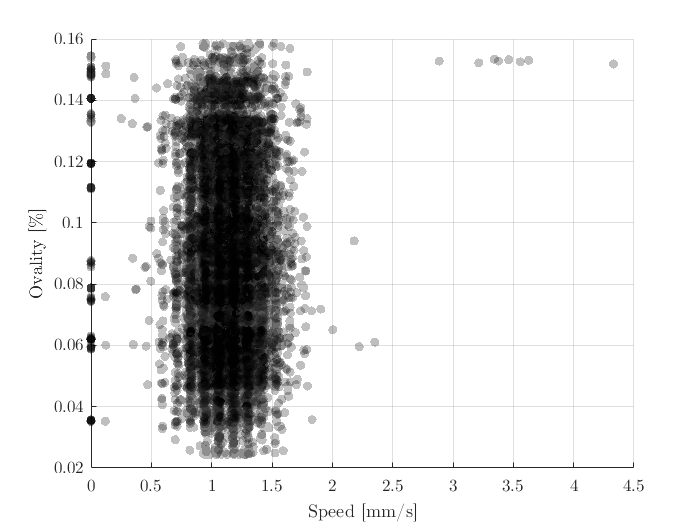
\includegraphics[width=0.8\linewidth, keepaspectratio]{speed-ovality}
	}
	\linebreak
	\subfloat[Effect of ovality on measured filament force \label{fig:O_f}]{%
		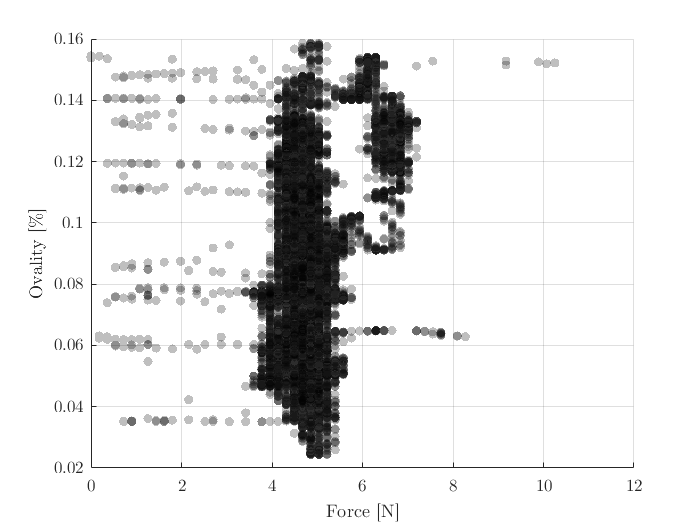
\includegraphics[width=0.8\linewidth, keepaspectratio]{force-ovality}
	}
	\caption{Effect of diameter on filament force and speed} \label{fig:ov_f_sp}
\end{figure}

\subsection{Data generation and preparation}\label{ssec:datag}

\subsection{ML system architecture, training, and validation}\label{ssec:MLA}

The following step of this work would involve using small subsets of the training data to test multiple models and algorithms in a reasonable amount of time. Performance metrics such as the Mean Square Error (MSE) or the Mean Absolute Error (MAE) would help narrow down the optimal candidate for each task \cite{Geron2019}. Depending on the outcome, the final architecture of the predictive system will be decided, including the algorithms for each segment of the machine learning pipeline if applicable. Ultimately, the final architecture of the system will be trained using the training data, and benchmarked against the validation set to check for inherent issues to the ML field, such as overfitting, and to assess the validity of the predicted outcome. The programming language of choice will be \emph{Python 3}, given its relative ease of syntax, open-source nature, as well as the availability of data science and ML libraries and resources such as \emph{NumPy, pandas, and TensorFlow}.


%______________________________________________________________________________________________
% Nomenclature introduced in this chapter:
\nomenclature[A]{ML}{Machine Learning}% 
\nomenclature[A]{SVM}{Support Vector Machines}%
\nomenclature[A]{NN}{Neural Network}%
\nomenclature[A]{MSE}{Mean Square Error}%
\nomenclature[A]{MAE}{Mean Absolute Error}%

% Symbols introduced in this chapter:
%\nomenclature[S]{$X_t$}{Tensile strength in the 1-1 direction \nomunit{$MPa$}}
\end{document}
                %\include{results}
                %\include{conclusions}
%               \include{examples}

		%Create Bibliography
		\cleardoublepage
        \phantomsection
		\addcontentsline{toc}{chapter}{Bibliography}
		\printbibliography		
        %Create Appendices
        
		\appendix
			% mg94.tex
\documentclass[main.tex]{subfiles}
\begin{document}
	\chapter{SABIC Cycolac MG94 Datasheet}\label{ch:mg94}

Reproduced from SABIC's Datasheet Document \cite{sabic2016}.
	
	\begin{figure}[h]
		\center
		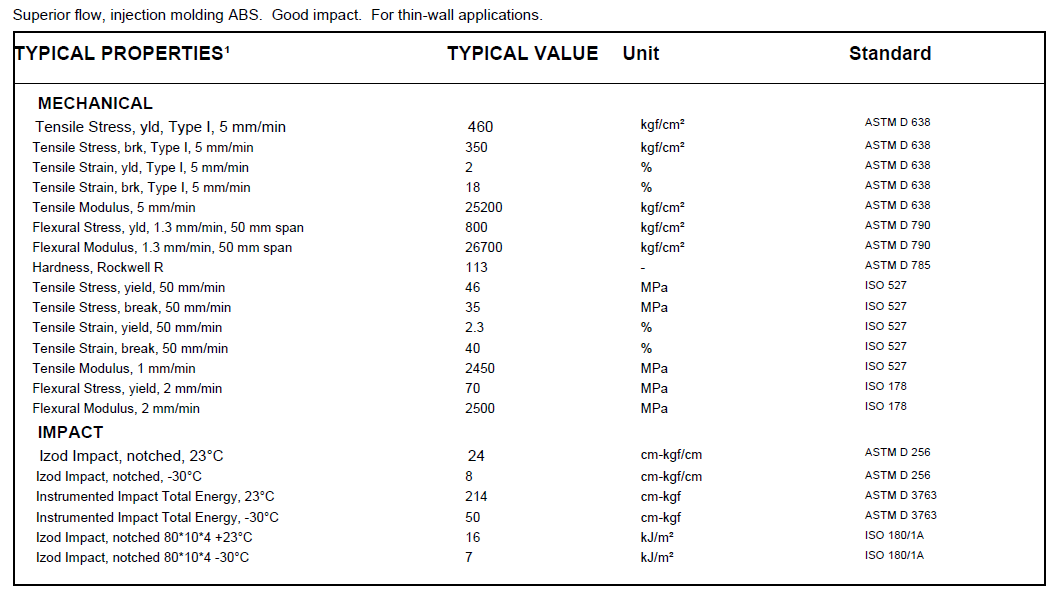
\includegraphics[width=\linewidth, keepaspectratio]{mg94_1}
		\label{fig:mg941}
	\end{figure}

	\begin{figure}[h]
		\center
		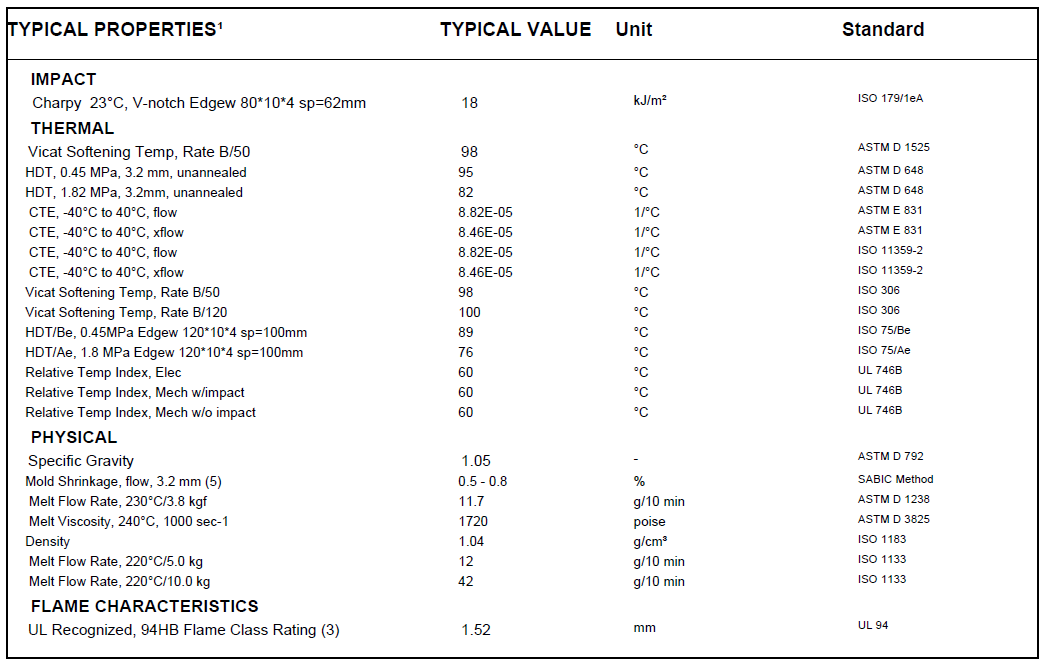
\includegraphics[width=\linewidth, keepaspectratio]{mg94_2}
		\label{fig:mg942}
	\end{figure}

	\begin{figure}[h]
	\center
	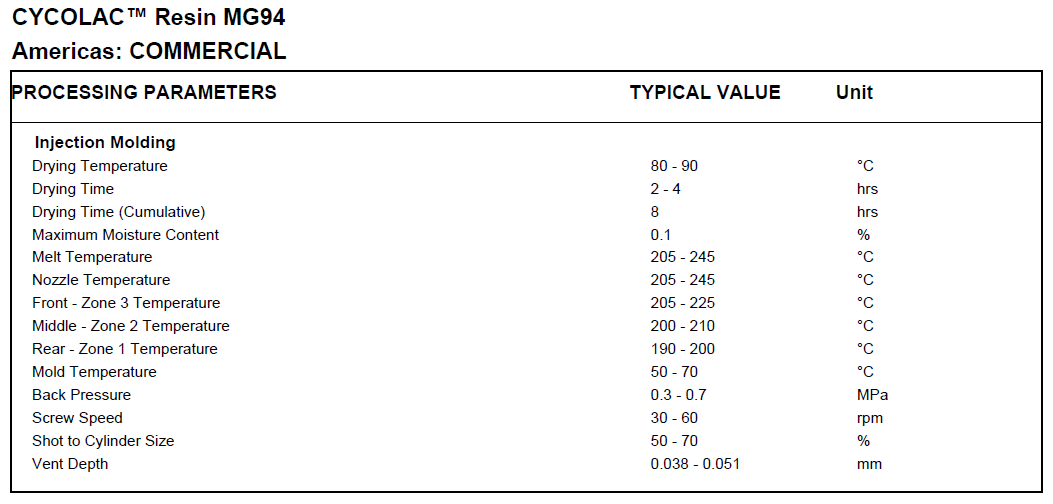
\includegraphics[width=\linewidth, keepaspectratio]{mg94_3}
	\label{fig:mg943}
	\end{figure}
\end{document}
			\pagestyle{fancy}
			%% fsurfcode.tex
\documentclass[main.tex]{subfiles}
\begin{document}
	\chapter{Failure Criterion Calculation Code}\label{ch:fsurfcode}
	\lstinputlisting[style=Matlab-editor, basicstyle=\mlttfamily\scriptsize]{FailureCriteria.m}
\end{document}
			%\include{data}
			%\include{surf}
			


        
\end{document}
